
%% bare_jrnl.tex
%% V1.4b
%% 2015/08/26
%% by Michael Shell
%% see http://www.michaelshell.org/
%% for current contact information.
%%
%% This is a skeleton file demonstrating the use of IEEEtran.cls
%% (requires IEEEtran.cls version 1.8b or later) with an IEEE
%% journal paper.
%%
%% Support sites:
%% http://www.michaelshell.org/tex/ieeetran/
%% http://www.ctan.org/pkg/ieeetran
%% and
%% http://www.ieee.org/

%%*************************************************************************
%% Legal Notice:
%% This code is offered as-is without any warranty either expressed or
%% implied; without even the implied warranty of MERCHANTABILITY or
%% FITNESS FOR A PARTICULAR PURPOSE! 
%% User assumes all risk.
%% In no event shall the IEEE or any contributor to this code be liable for
%% any damages or losses, including, but not limited to, incidental,
%% consequential, or any other damages, resulting from the use or misuse
%% of any information contained here.
%%
%% All comments are the opinions of their respective authors and are not
%% necessarily endorsed by the IEEE.
%%
%% This work is distributed under the LaTeX Project Public License (LPPL)
%% ( http://www.latex-project.org/ ) version 1.3, and may be freely used,
%% distributed and modified. A copy of the LPPL, version 1.3, is included
%% in the base LaTeX documentation of all distributions of LaTeX released
%% 2003/12/01 or later.
%% Retain all contribution notices and credits.
%% ** Modified files should be clearly indicated as such, including  **
%% ** renaming them and changing author support contact information. **
%%*************************************************************************


% *** Authors should verify (and, if needed, correct) their LaTeX system  ***
% *** with the testflow diagnostic prior to trusting their LaTeX platform ***
% *** with production work. The IEEE's font choices and paper sizes can   ***
% *** trigger bugs that do not appear when using other class files.       ***                          ***
% The testflow support page is at:
% http://www.michaelshell.org/tex/testflow/



\documentclass[journal]{IEEEtran}
%
% If IEEEtran.cls has not been installed into the LaTeX system files,
% manually specify the path to it like:
% \documentclass[journal]{../sty/IEEEtran}





% Some very useful LaTeX packages include:
% (uncomment the ones you want to load)


% *** MISC UTILITY PACKAGES ***
%
%\usepackage{ifpdf}
% Heiko Oberdiek's ifpdf.sty is very useful if you need conditional
% compilation based on whether the output is pdf or dvi.
% usage:
% \ifpdf
%   % pdf code
% \else
%   % dvi code
% \fi
% The latest version of ifpdf.sty can be obtained from:
% http://www.ctan.org/pkg/ifpdf
% Also, note that IEEEtran.cls V1.7 and later provides a builtin
% \ifCLASSINFOpdf conditional that works the same way.
% When switching from latex to pdflatex and vice-versa, the compiler may
% have to be run twice to clear warning/error messages.






% *** CITATION PACKAGES ***
%
%\usepackage{cite}
% cite.sty was written by Donald Arseneau
% V1.6 and later of IEEEtran pre-defines the format of the cite.sty package
% \cite{} output to follow that of the IEEE. Loading the cite package will
% result in citation numbers being automatically sorted and properly
% "compressed/ranged". e.g., [1], [9], [2], [7], [5], [6] without using
% cite.sty will become [1], [2], [5]--[7], [9] using cite.sty. cite.sty's
% \cite will automatically add leading space, if needed. Use cite.sty's
% noadjust option (cite.sty V3.8 and later) if you want to turn this off
% such as if a citation ever needs to be enclosed in parenthesis.
% cite.sty is already installed on most LaTeX systems. Be sure and use
% version 5.0 (2009-03-20) and later if using hyperref.sty.
% The latest version can be obtained at:
% http://www.ctan.org/pkg/cite
% The documentation is contained in the cite.sty file itself.






% *** GRAPHICS RELATED PACKAGES ***
%
\ifCLASSINFOpdf
  % \usepackage[pdftex]{graphicx}
  % declare the path(s) where your graphic files are
  % \graphicspath{{../pdf/}{../jpeg/}}
  % and their extensions so you won't have to specify these with
  % every instance of \includegraphics
  % \DeclareGraphicsExtensions{.pdf,.jpeg,.png}
\else
  % or other class option (dvipsone, dvipdf, if not using dvips). graphicx
  % will default to the driver specified in the system graphics.cfg if no
  % driver is specified.
  % \usepackage[dvips]{graphicx}
  % declare the path(s) where your graphic files are
  % \graphicspath{{../eps/}}
  % and their extensions so you won't have to specify these with
  % every instance of \includegraphics
  % \DeclareGraphicsExtensions{.eps}
\fi
% graphicx was written by David Carlisle and Sebastian Rahtz. It is
% required if you want graphics, photos, etc. graphicx.sty is already
% installed on most LaTeX systems. The latest version and documentation
% can be obtained at: 
% http://www.ctan.org/pkg/graphicx
% Another good source of documentation is "Using Imported Graphics in
% LaTeX2e" by Keith Reckdahl which can be found at:
% http://www.ctan.org/pkg/epslatex
%
% latex, and pdflatex in dvi mode, support graphics in encapsulated
% postscript (.eps) format. pdflatex in pdf mode supports graphics
% in .pdf, .jpeg, .png and .mps (metapost) formats. Users should ensure
% that all non-photo figures use a vector format (.eps, .pdf, .mps) and
% not a bitmapped formats (.jpeg, .png). The IEEE frowns on bitmapped formats
% which can result in "jaggedy"/blurry rendering of lines and letters as
% well as large increases in file sizes.
%
% You can find documentation about the pdfTeX application at:
% http://www.tug.org/applications/pdftex





% *** MATH PACKAGES ***
%
%\usepackage{amsmath}
% A popular package from the American Mathematical Society that provides
% many useful and powerful commands for dealing with mathematics.
%
% Note that the amsmath package sets \interdisplaylinepenalty to 10000
% thus preventing page breaks from occurring within multiline equations. Use:
%\interdisplaylinepenalty=2500
% after loading amsmath to restore such page breaks as IEEEtran.cls normally
% does. amsmath.sty is already installed on most LaTeX systems. The latest
% version and documentation can be obtained at:
% http://www.ctan.org/pkg/amsmath





% *** SPECIALIZED LIST PACKAGES ***
%
%\usepackage{algorithmic}
% algorithmic.sty was written by Peter Williams and Rogerio Brito.
% This package provides an algorithmic environment fo describing algorithms.
% You can use the algorithmic environment in-text or within a figure
% environment to provide for a floating algorithm. Do NOT use the algorithm
% floating environment provided by algorithm.sty (by the same authors) or
% algorithm2e.sty (by Christophe Fiorio) as the IEEE does not use dedicated
% algorithm float types and packages that provide these will not provide
% correct IEEE style captions. The latest version and documentation of
% algorithmic.sty can be obtained at:
% http://www.ctan.org/pkg/algorithms
% Also of interest may be the (relatively newer and more customizable)
% algorithmicx.sty package by Szasz Janos:
% http://www.ctan.org/pkg/algorithmicx




% *** ALIGNMENT PACKAGES ***
%
%\usepackage{array}
% Frank Mittelbach's and David Carlisle's array.sty patches and improves
% the standard LaTeX2e array and tabular environments to provide better
% appearance and additional user controls. As the default LaTeX2e table
% generation code is lacking to the point of almost being broken with
% respect to the quality of the end results, all users are strongly
% advised to use an enhanced (at the very least that provided by array.sty)
% set of table tools. array.sty is already installed on most systems. The
% latest version and documentation can be obtained at:
% http://www.ctan.org/pkg/array


% IEEEtran contains the IEEEeqnarray family of commands that can be used to
% generate multiline equations as well as matrices, tables, etc., of high
% quality.




% *** SUBFIGURE PACKAGES ***
%\ifCLASSOPTIONcompsoc
%  \usepackage[caption=false,font=normalsize,labelfont=sf,textfont=sf]{subfig}
%\else
%  \usepackage[caption=false,font=footnotesize]{subfig}
%\fi
% subfig.sty, written by Steven Douglas Cochran, is the modern replacement
% for subfigure.sty, the latter of which is no longer maintained and is
% incompatible with some LaTeX packages including fixltx2e. However,
% subfig.sty requires and automatically loads Axel Sommerfeldt's caption.sty
% which will override IEEEtran.cls' handling of captions and this will result
% in non-IEEE style figure/table captions. To prevent this problem, be sure
% and invoke subfig.sty's "caption=false" package option (available since
% subfig.sty version 1.3, 2005/06/28) as this is will preserve IEEEtran.cls
% handling of captions.
% Note that the Computer Society format requires a larger sans serif font
% than the serif footnote size font used in traditional IEEE formatting
% and thus the need to invoke different subfig.sty package options depending
% on whether compsoc mode has been enabled.
%
% The latest version and documentation of subfig.sty can be obtained at:
% http://www.ctan.org/pkg/subfig




% *** FLOAT PACKAGES ***
%
%\usepackage{fixltx2e}
% fixltx2e, the successor to the earlier fix2col.sty, was written by
% Frank Mittelbach and David Carlisle. This package corrects a few problems
% in the LaTeX2e kernel, the most notable of which is that in current
% LaTeX2e releases, the ordering of single and double column floats is not
% guaranteed to be preserved. Thus, an unpatched LaTeX2e can allow a
% single column figure to be placed prior to an earlier double column
% figure.
% Be aware that LaTeX2e kernels dated 2015 and later have fixltx2e.sty's
% corrections already built into the system in which case a warning will
% be issued if an attempt is made to load fixltx2e.sty as it is no longer
% needed.
% The latest version and documentation can be found at:
% http://www.ctan.org/pkg/fixltx2e


%\usepackage{stfloats}
% stfloats.sty was written by Sigitas Tolusis. This package gives LaTeX2e
% the ability to do double column floats at the bottom of the page as well
% as the top. (e.g., "\begin{figure*}[!b]" is not normally possible in
% LaTeX2e). It also provides a command:
%\fnbelowfloat
% to enable the placement of footnotes below bottom floats (the standard
% LaTeX2e kernel puts them above bottom floats). This is an invasive package
% which rewrites many portions of the LaTeX2e float routines. It may not work
% with other packages that modify the LaTeX2e float routines. The latest
% version and documentation can be obtained at:
% http://www.ctan.org/pkg/stfloats
% Do not use the stfloats baselinefloat ability as the IEEE does not allow
% \baselineskip to stretch. Authors submitting work to the IEEE should note
% that the IEEE rarely uses double column equations and that authors should try
% to avoid such use. Do not be tempted to use the cuted.sty or midfloat.sty
% packages (also by Sigitas Tolusis) as the IEEE does not format its papers in
% such ways.
% Do not attempt to use stfloats with fixltx2e as they are incompatible.
% Instead, use Morten Hogholm'a dblfloatfix which combines the features
% of both fixltx2e and stfloats:
%
% \usepackage{dblfloatfix}
% The latest version can be found at:
% http://www.ctan.org/pkg/dblfloatfix




%\ifCLASSOPTIONcaptionsoff
%  \usepackage[nomarkers]{endfloat}
% \let\MYoriglatexcaption\caption
% \renewcommand{\caption}[2][\relax]{\MYoriglatexcaption[#2]{#2}}
%\fi
% endfloat.sty was written by James Darrell McCauley, Jeff Goldberg and 
% Axel Sommerfeldt. This package may be useful when used in conjunction with 
% IEEEtran.cls'  captionsoff option. Some IEEE journals/societies require that
% submissions have lists of figures/tables at the end of the paper and that
% figures/tables without any captions are placed on a page by themselves at
% the end of the document. If needed, the draftcls IEEEtran class option or
% \CLASSINPUTbaselinestretch interface can be used to increase the line
% spacing as well. Be sure and use the nomarkers option of endfloat to
% prevent endfloat from "marking" where the figures would have been placed
% in the text. The two hack lines of code above are a slight modification of
% that suggested by in the endfloat docs (section 8.4.1) to ensure that
% the full captions always appear in the list of figures/tables - even if
% the user used the short optional argument of \caption[]{}.
% IEEE papers do not typically make use of \caption[]'s optional argument,
% so this should not be an issue. A similar trick can be used to disable
% captions of packages such as subfig.sty that lack options to turn off
% the subcaptions:
% For subfig.sty:
% \let\MYorigsubfloat\subfloat
% \renewcommand{\subfloat}[2][\relax]{\MYorigsubfloat[]{#2}}
% However, the above trick will not work if both optional arguments of
% the \subfloat command are used. Furthermore, there needs to be a
% description of each subfigure *somewhere* and endfloat does not add
% subfigure captions to its list of figures. Thus, the best approach is to
% avoid the use of subfigure captions (many IEEE journals avoid them anyway)
% and instead reference/explain all the subfigures within the main caption.
% The latest version of endfloat.sty and its documentation can obtained at:
% http://www.ctan.org/pkg/endfloat
%
% The IEEEtran \ifCLASSOPTIONcaptionsoff conditional can also be used
% later in the document, say, to conditionally put the References on a 
% page by themselves.




% *** PDF, URL AND HYPERLINK PACKAGES ***
%
%\usepackage{url}
% url.sty was written by Donald Arseneau. It provides better support for
% handling and breaking URLs. url.sty is already installed on most LaTeX
% systems. The latest version and documentation can be obtained at:
% http://www.ctan.org/pkg/url
% Basically, \url{my_url_here}.




% *** Do not adjust lengths that control margins, column widths, etc. ***
% *** Do not use packages that alter fonts (such as pslatex).         ***
% There should be no need to do such things with IEEEtran.cls V1.6 and later.
% (Unless specifically asked to do so by the journal or conference you plan
% to submit to, of course. )


\usepackage{graphicx}  %Required
\frenchspacing  %Required
\setlength{\pdfpagewidth}{8.5in}  %Required
\setlength{\pdfpageheight}{11in}  %Required
%PDF Info Is Required:
  \pdfinfo{
/Title (2019 Formatting Instructions for Authors Using LaTeX)
/Author (AAAI Press Staff)}
\usepackage[noend]{algpseudocode}
\usepackage{algorithm,amsmath}
\usepackage{mathtools}
\usepackage{newtxtext,newtxmath}
\usepackage[utf8]{inputenc}
\usepackage{adjustbox}

\let\openbox\relax
\usepackage{amsthm}
\usepackage{comment}
\usepackage[utf8]{inputenc}
\usepackage{subfig}
\usepackage[dvipsnames]{xcolor}
\newcommand*{\R}{\mathbb{R}}
\newcommand*{\Po}{\text{Prox}}
\newcommand*{\Am}{\text{argmin}}
\newcommand*{\E}{\mathbb{E}}
\newcommand*{\VRG}{\,\tilde{\nabla}_k^s}
\newcommand{\norm}[1]{\left\lVert#1\right\rVert}
\newcommand{\Iprod}[2]{\left\langle #1,#2\right\rangle}
\newcommand\myeq[2]{\mathrel{\stackrel{{{#1}}}{#2}}}
\newcommand{\abs}[1]{\left|#1\right|}

\renewcommand{\algorithmicrequire}{
\textbf{Input:}}
\renewcommand{\algorithmicensure}{\textbf{Output:}}
\newcommand{\Initialize}{\textbf{Initialize:}{\,}}
\newcommand{\Input}{\textbf{Input:}{\,}}
\newcommand{\Output}{\textbf{Output:}{\,}}


\newtheorem{theorem}{Theorem}
\newtheorem{lemma}[theorem]{Lemma}
\newtheorem{conjecture}[theorem]{Conjecture}
\newtheorem{condition}[theorem]{Condition}
\newtheorem{claim}[theorem]{Claim}
\newtheorem{question}[theorem]{Question}
\newtheorem{corollary}[theorem]{Corollary} 
\newtheorem{definition}{Definition}
\newtheorem{statement}[theorem]{Statement}
\newtheorem{notation}[theorem]{Notation} 
\newtheorem{remark}{Remark}
\newtheorem{assumption}{Assumption}
\setcounter{secnumdepth}{0}  
\newcommand{\keepcomment}{1}% Remove comment
\AtBeginDocument{\ifnum\keepcomment=1
  \excludecomment{comment}
\else
  \includecomment{comment}
\fi}
\allowdisplaybreaks
\includeonly{sub1}

% correct bad hyphenation here
\hyphenation{op-tical net-works semi-conduc-tor}


\begin{document}
%
% paper title
% Titles are generally capitalized except for words such as a, an, and, as,
% at, but, by, for, in, nor, of, on, or, the, to and up, which are usually
% not capitalized unless they are the first or last word of the title.
% Linebreaks \\ can be used within to get better formatting as desired.
% Do not put math or special symbols in the title.
\title{Efficient Zeroth-Order Proximal Stochastic Method for Nonconvex Nonsmooth Black-Box Optimization}
%
%
% author names and IEEE memberships
% note positions of commas and nonbreaking spaces ( ~ ) LaTeX will not break
% a structure at a ~ so this keeps an author's name from being broken across
% two lines.
% use \thanks{} to gain access to the first footnote area
% a separate \thanks must be used for each paragraph as LaTeX2e's \thanks
% was not built to handle multiple paragraphs
%

\author{Ehsan~Kazemi, ~Liqiang~Wang,~\IEEEmembership{Member,~IEEE}
%        John~Doe,~\IEEEmembership{Fellow,~OSA,}
%        and~Jane~Doe,~\IEEEmembership{Life~Fellow,~IEEE}% <-this % stops a space
\thanks{E. Kazemi and L. Wang are  with  the  Department of Computer Science,  University of Central Florida, Orlando, Florida, USA (e-mail: ehsan\_ kazemy@knights.ucf.edu; lwang@cs.ucf.edu). D. Fan is with the School of Electrical, Computer and Energy Engineering, Arizona State University (email: dfan@asu.edu). The work was supported in part by NSF-1741431.}% <-this % stops a space
%\thanks{J. Doe and J. Doe are with Anonymous University.}% <-this % stops a space
%\thanks{Manuscript received April 19, 2005; revised August 26, 2015.}
}

% note the % following the last \IEEEmembership and also \thanks - 
% these prevent an unwanted space from occurring between the last author name
% and the end of the author line. i.e., if you had this:
% 
% \author{....lastname \thanks{...} \thanks{...} }
%                     ^------------^------------^----Do not want these spaces!
%
% a space would be appended to the last name and could cause every name on that
% line to be shifted left slightly. This is one of those "LaTeX things". For
% instance, "\textbf{A} \textbf{B}" will typeset as "A B" not "AB". To get
% "AB" then you have to do: "\textbf{A}\textbf{B}"
% \thanks is no different in this regard, so shield the last } of each \thanks
% that ends a line with a % and do not let a space in before the next \thanks.
% Spaces after \IEEEmembership other than the last one are OK (and needed) as
% you are supposed to have spaces between the names. For what it is worth,
% this is a minor point as most people would not even notice if the said evil
% space somehow managed to creep in.



% The paper headers
%\markboth{IEEE TRANSACTIONS ON CYBERNETICS}%
%{Shell \MakeLowercase{\textit{et al.}}: Bare Demo of IEEEtran.cls for IEEE Journals}
% The only time the second header will appear is for the odd numbered pages
% after the title page when using the twoside option.
% 
% *** Note that you probably will NOT want to include the author's ***
% *** name in the headers of peer review papers.                   ***
% You can use \ifCLASSOPTIONpeerreview for conditional compilation here if
% you desire.




% If you want to put a publisher's ID mark on the page you can do it like
% this:
%\IEEEpubid{0000--0000/00\$00.00~\copyright~2015 IEEE}
% Remember, if you use this you must call \IEEEpubidadjcol in the second
% column for its text to clear the IEEEpubid mark.



% use for special paper notices
%\IEEEspecialpapernotice{(Invited Paper)}




% make the title area
\maketitle

% As a general rule, do not put math, special symbols or citations
% in the abstract or keywords.
\begin{abstract}
Proximal gradient method has an important role
in solving nonsmooth composite optimization problems. However, in some machine learning problems related to black-box optimization models proximal gradient method could not be leveraged, where explicit gradient forms are difficult or infeasible to obtain. While first order methods are not suited for solving black-box optimization problems, zeroth-order (ZO) optimization methods can address these problems efficiently. Several varieties of zeroth-order variance reduced stochastic (ZO-SVRG) algorithms have recently been introduced for nonconvex optimization based on the first-order techniques of stochastic variance reduction. However, all existing ZO-SVRG type  algorithms suffer from a slowdown and increase in function query complexities up  to a small-degree  polynomial  of  the  problem  size. To fill this gap, we propose a new stochastic gradient algorithm in the gradient-free regime for optimizing nonconvex, nonsmooth finite-sum problems, called ZO-PSVRG+. The analysis of ZO-PSVRG+ recovers several existing convergence results and improves their ZO oracle and proximal oracle calls. Furthermore, we prove that ZO-PSVRG+ under Polyak-Łojasiewicz condition in contrast to the existent ZO-SVRG type methods obtain a global linear convergence for a wide range of minibatch sizes. Our empirical experiments on black-box binary classification and black-box adversarial attack from black-box neural networks demonstrate that the studied algorithms under our new analysis exhibit superior performance and faster convergence to a solution of high accuracy with a lower query complexity compared to state-of-the-art ZO optimization methods for nonconvex nonsmooth problems.
\end{abstract}

% Note that keywords are not normally used for peerreview papers.
\begin{IEEEkeywords}
Block-box optimization, zeroth-order gradient estimator (ZO), stochastic variance reduced gradient descent (SVRG), adversarial examples.
\end{IEEEkeywords}






% For peer review papers, you can put extra information on the cover
% page as needed:
% \ifCLASSOPTIONpeerreview
% \begin{center} \bfseries EDICS Category: 3-BBND \end{center}
% \fi
%
% For peerreview papers, this IEEEtran command inserts a page break and
% creates the second title. It will be ignored for other modes.
\IEEEpeerreviewmaketitle

\section{Introduction}
In this paper, we consider the nonsmooth nonconvex optimization problems of the following form
\begin{equation}\label{problem}
\min_{x\in\R^d} F(x) =  f(x) + h(x),\,\,\,f(x):=\frac{1}{n}\sum_{i=1}^n f_i(x)
\end{equation}
where each $f_i(x)$ is possibly nonconvex and smooth function, and $h(x)$ is a nonsmooth convex function such as $l_1$-norm regularizer. 
The general structure \eqref{problem} covers
numerous machine learning areas, ranged from neural networks to  generalized linear models  
 and from convex problems like  SVM  and Lasso to highly nonconvex optimization including minimizing loss function for deep learning. We will investigate and explore a set of accelerated variance reduced stochastic zeroth-order (SZO) optimization algorithms for \eqref{problem}. Stochastic variance reduced gradient
(SVRG) is a generic and powerful methodology to decrease the variance induced by stochastic sampling \cite{johnson2013accelerating,reddi2016stochastic,nitanda2016accelerated,allen2016improved,lei2017non}. As a result of reduction in variance, it enhances the rate of convergence for stochastic gradient descent (SGD) complexity by a factor of $O(1/{\epsilon})$. To reduce the variance in SZO optimization, one may apply the comparable concepts and similar ideas in the first-order methods. 
\iffalse
\subsection{Background in research}
In recent years, there has been thorough studies for convex problems of the form \eqref{problem} (see e.g., \cite{nesterov2013gradient}, \cite{xiao2014proximal,defazio2014saga,lan2017optimal,allen2017katyusha}. 
In particular, in \cite{beck2009fast} a fast-converging class of proximal gradient (PG) schemes for problems with convex structure based on Nesterov's momentum acceleration are designed.  
\cite{xiao2014proximal} developed an algorithm called Prox-SVRG for large-scale problems, which
obtains a linear rate of convergence when each  $f_i$ is strongly-convex. Several stochastic PG methods were developed in \cite{bertsekas2011incremental,xiao2014proximal}  to deal with the large-scale convex problems. Because of growing applications of deep neural networks, recently the studies for nonconvex case have been noticeably growing. Nevertheless, for the generic nonsmooth nonconvex problems, the analysis is still rather sparse.  \cite{li2015accelerated} introduced a set of fast-converging PG algorithms for nonconvex structure problems. Similarly, \cite{ghadimi2016accelerated,reddi2016proximal} studied stochastic PG methods for nonconvex optimization.
Recently, \cite{li2018simple} designed an algorithm by extending the results from \cite{reddi2016proximal}, leading to an improved iteration complexity for stochastic gradient method. 
\fi

The major adversity for these accelerated methods is their designs on involving first-order information. Nevertheless, there are circumstances where the first-order gradient evaluations are computationally unrealizable, costly, or unachievable, while zeroth-order information (function information) are accessible. For instance, in online auctions and advertisement
selections, only zeroth-order information in the form of responses to the queries is accessible \cite{wibisono2012finite}. Similarly, in predictions with stochastic structure, computing the derivatives is possibly complicated or prohibited, while the functional estimations of foreseen frameworks are achievable  \cite{sokolov2016stochastic}. 
As an example, in bandit \cite{shamir2017optimal} and black-box intelligence \cite{chen2017zoo} settings, only the loss function evaluations are accessible as the derivatives cannot be calculated directly. 
Thus, the derivative-free  optimization algorithms \cite{nesterov2017random} are viable options to tackle these issues. This procedure approximates the full gradient via gradient evaluator based on only the function estimations which end up in derivative-free optimization \cite{brent2013algorithms,spall2005introduction}. 
We describe the minimization problem \eqref{problem} in this particular setting as stochastic proximal zeroth-order optimization.
\iffalse
Recently, zeroth-order optimization has attracted significant attention due to its diverse applications, e.g., black-box adversarial attacks on deep neural networks (DNNs)\cite{kurakin2016adversarial,papernot2017practical,chen2017zoo}, reinforcement learning \cite{choromanski2018structured} and structured prediction \cite{taskar2005learning}.
Further applications cover time-varying constrained networks with restricted computation capacity \cite{chen2019bandit,liu2017zeroth}, and model inference with black-box setting \cite{fu2002optimization,lian2016comprehensive}. 
\fi
\iffalse
Currently, there are only a few number of zeroth-order stochastic methods
for solving problem \eqref{problem}, e.g., \cite{ghadimi2016accelerated} and \cite{huang2019faster}. In particular, in \cite{ghadimi2016accelerated} a zeroth-order proximal stochastic gradient method has been analyzed. Nevertheless, as a result of the high variance of zeroth-order gradient approximation based on random sampling and vector sampling for two point derivative calculations, the iteration complexity of RSPGE (i.e., $O(\frac{d}{\epsilon^2})$) is notably worse than the best known rate $O(\frac{d}{{\epsilon}})$ for zeroth-order stochastic optimization. A major issue in the advancement of SZO algorithms for solving  \eqref{problem} is the order of the required number of function queries, namely SZO calls or iteration complexity. While the existing zeroth-order methods based upon SVRG algorithms have higher convergence rate, the complexity of their function calls are all greater than each of ZO-GD and ZO-SGD. They also rely on a very small and some often diminishing stepsize $O(\frac{1}{d})$. To perform an elaborated analysis, the term related to the dimension of the problem in the convergence studies (i.e., $d$) is a key factor with high impact on the efficiency of SZO optimization. \cite{ji2019improved} refined the ZO estimations to achieve an improved ZO complexity and enhanced convergence rate. However, their improved analysis is only for smooth functions based on a complicated parameter selection and it is only valid for large minibatch sizes.
We design an accelerated ZO proximal variants by applying variance reduced gradient approximation for nonsmooth composite optimization. This provides a lower iteration complexity towards $O(1/\epsilon )$, which is to our knowledge the best iteration complexity bound obtained thus far for proximal ZO stochastic optimization with nonconvex structure.
This demonstrates an improvement for ZO iteration complexity up to a factor of ${d}$.
\fi
We compared the results from our analysis and other comparable SZO algorithms in Table \ref{table-compare}. It indicates
that RGF has the largest query complexity and yet has the worst convergence rate. ZO-SVRG-coord
and ZO-ProxSVRG/SAGA provide an improved rate of convergence $O(d/\epsilon )$ due to using variance reduction techniques. On the other hand, existing SVRG type zeroth-order algorithms are affected by worse function query complexities compared with RSPGF, while our algorithm, ZO-PSVRG+, could achieve better trade-offs between the convergence rate and the query complexity.

\iffalse
\section{Main Challenge}
Despite the fact that proximal SVRG has indicated a huge promise for first-order algorithms, utilizing identical concepts to ZO optimization is not effortless. 
Due to the perturbation induced by ZO gradient estimation, SZO algorithms have complex joint structures, which make their analysis difficult in many settings. The other major difficulty is due to the fact that ProxSVRG is based upon the notion that stochastic gradient is an unbiased approximation of the actual full gradient, which is not retained in the ZO case. Thus, it is a challenging question if the proximal ZO stochastic variance reduced gradient could accelerate the convergence of proximal ZO algorithms with arbitrary minibatch sizes. In this paper, we plan to address this question and in particular fill the void between
SZO optimization and ProxSVRG by improving the complexity of exiting ZO variance reduced methods for problem \eqref{problem}.
\fi


\section{Main contributions}
We present a novel analysis beyond the existing convergence studies introduced in \cite{liu2018zeroth,ji2019improved}, and
prove that ZO-PSVRG+ based on  our new analysis surpasses other state-of-the-art SVRG-type zeroth-order methods as well as RSPGF.
We concentrate on several important debatable questions in these methods. Particularly, we somewhat address the open question if the dependence on the dimension $d$ for the convergence analysis proposed in \cite{liu2018zeroth} is optimal. Our work provides an inclusive analysis on how ZO gradient approximations influence ProxSVRG on both  convergence rate and function query complexity. This
is performed based on the novel structure of recently introduced SZO algorithms.
Note our analysis does not rely on bounded gradient assumption in \cite{ghadimi2016accelerated,huang2019faster}.
The convergence results are declared with respect to the number of stochastic zeroth-order (SZO) queries and proximal oracle (PO) calls. 
Based on our new analysis, we summarize the following results from this paper:

1) Our analysis yields iteration complexity $O(\frac{1}{{\epsilon}})$ corresponding to $O(\frac{d}{\epsilon^2})$ of RSPGF \cite{ghadimi2016accelerated}  and $O(\frac{d}{\epsilon})$ of ZO-ProxSVRG/SAGA  \cite{huang2019faster} (the existing variance-reduce SZO proximal algorithm for solving nonconvex nonsmooth problems).  
Thus, our results have better or no dependence on
$d$ in contrast to the existing proximal variance-reduced SZO methods. ZO-PSVRG+ also matches the best result achieved by ZO-SVRG-Coord-Rand with minibatch size $b = d n^{2/3}$ and epoch size $m = n^{1/3}$ in \cite{ji2019improved}, while our results are valid for unspecified minibatch sizes as detailed in the following sections.  
Indeed, it is necessary to analyze and study the convergence behavior of SZO optimization with minibatchs of single or moderate sizes, as practically many machine learning models are trained with intermediate minibatch sizes.


2) The convergence analysis for ZO-PSVRG+ is straightforward in contrast to  ZO-SVRG-Coord in \cite{liu2018zeroth,ji2019improved}, and yields simpler proofs. Our analysis achieves new iteration complexity bounds and improves the effectiveness of  all the existing ZO-SVRG-based algorithms in addition to RSPGF for nonconvex nonsmooth composite optimization and it provides the best results to our best knowledge (see Table \ref{table-compare}). Note that the convergence studies for RSPGF and ZO-ProxSVRG/SAGA rely on bounded gradient assumption, which is not our working assumption in this paper.


3) For the nonconvex functions under Polyak-Łojasiewicz condition \cite{polyak1963gradient}, we show that ZO-PSVRG+
obtains a global linear rate of convergence  equivalent to first-order ProxSVRG. Thus, ZO-PSVRG+ can certainly achieve linear convergence in some zones without restarting. To the best of
our knowledge, this is the first paper that leverages the PL condition for improving the convergence of of ZO-ProxSVRG for problem \eqref{problem} with arbitrary minibatch sizes. This analysis generalizes the results of \cite{duchi2015optimal} while  shows linear convergence versus the sublinear convergence rate in their paper.
In \cite{ji2019improved}, the authors show that  ZO-SPIDER-Coord achieves linear convergence under PL condition but only for the minibatch size $b = O(n^{1/2})$.  Note that due to both computational and statistical efficiency, convergence analysis for minibatchs of moderate sizes is demanding. Also see the remarks after Theorem \ref{PL-Zoo-rand} for more details. 

Finally, to demonstrate the efficiency and adaptability of our approach to achieve a balance between the rate of convergence and the number of SZO queries, we perform some
experimental evaluations for two distinct applications: black-box binary classification and universal adversarial
attacks on black-box deep neural network models. The empirical results and
theoretical investigations verify the effectiveness of our algorithms.

%\iffalse
%\section{Related Works}
%Derivative-free (zeroth-order) methods have been efficiently utilized for solving numerous machine learning problems when the computation of the true gradient is infeasible. In ZO algorithms, a full gradient is generally estimated based on either a one-point or a two-point gradient approximation. The one-point estimator obtains a gradient estimate $\hat{\nabla} f(x)$ by probing $f$ at a single random point near to $x$ \cite{flaxman2005online,shamir2013complexity},  while the two-point estimator computes a difference of two random function probings \cite{agarwal2010optimal,nesterov2017random}. In this paper, we concentrate on the two-point gradient approximation since it has a lower variance and thus amends the iteration complexity of ZO algorithms. \cite{nesterov2017random} proposed several stochastic derivative-free
%algorithms by employing Gaussian smoothing method.  A zeroth-order mirror descent algorithm is analyzed in \cite{duchi2015optimal}. 
%More recently, \cite{yu2018generic,dvurechensky2018accelerated} introduced some accelerated zeroth-order algorithms for convex optimization. The recent studies confirmed that ZO algorithms typically agree with the complexity of first-order algorithms up to a small-degree polynomial of the problem size $d$.
%
%These zeroth-order algorithms mostly target (strongly) convex problems. Despite the extensive studies for the convex structures, the studies for nonconvex ZO methods are relatively limited.  Essentially, there are many nonconvex machine learning application, where the explicit derivatives are not accessible, e.g., nonconvex black-box learning problems \cite{chen2017zoo,liu2018zeroth}. Thus, developing zeroth-order stochastic methods for the nonconvex optimization is indeed demanding.
%\cite{ghadimi2013stochastic} and \cite{nesterov2011random} proposed ZO-GD and
%its corresponding stochastic algorithm ZO-SGD, respectively. \cite{liu2018stochastic} introduced a variance reduced stochastic zeroth-order method with  Gaussian smoothing. More recently, \cite{liu2018zeroth} presented a thorough analysis based on SVRG algorithms. \cite{ji2019improved} elaborated the results in \cite{liu2018zeroth} and achieved improved bounds based on a complicated parameter selection, however their improvements rely on large minibatch sizes. 
%Recently, for nonsmooth nonconvex problems \cite{huang2019faster} provided two algorithms called ZO-ProxSVRG and ZO-ProxSAGA, which are based on the well-known variance reduction techniques ProxSVRG and ProxSAGA \cite{reddi2016proximal}. Before that,  \cite{ghadimi2016accelerated} also considered the stochastic case (here we denote
%it as RSPGF). However, RSPGF requires increasing or large minibatch sizes i.e., $\Omega(1/\epsilon)$. Note that due to the
%growing minibatch sizes, RSPGF may change to deterministic proximal gradient descent (ZO-ProxGD) after few iterations. Further, \cite{liu2018stochastic} have also analyzed a zeroth-order algorithm for solving nonconvex nonsmooth problems, which are different from problem \eqref{problem}.
%In order to deal with the large-scale problems, several asynchronous stochastic zeroth-order algorithms have been studied, e.g., \cite{gu2018inexact,lian2016comprehensive,gu2018faster}.
%In \cite{lian2016comprehensive}, an asynchronous ZO stochastic coordinate
%descent (ZO-SCD) was designed with a convergence rate of $O(d/\epsilon^2)$.
%The convergence rate of asynchronous SZO further improved in \cite{gu2018faster} 
% by integrating SVRG techniques with stochastic coordinate descent method.
%  
%Even though the abovementioned zeroth-order stochastic algorithms can effectively solve the problems with nonconvex structure, there are limited number of zeroth-order stochastic methods for nonconvex nonsmooth composite problems. We emphasize that, in contrast to existing ZO proximal methods, our analysis do not require bounded gradient assumption, which is not valid for many unconstrained optimization problems. 
%It should be highlighted that computing full-gradient may not be effective for large-scale machine learning problems. Thus, we focus on studying a more general framework of ZO-ProxSVRG with different gradient estimators.
%\fi
\begin{table*}[t]
\begin{center}
\begin{tabular}{ |l|l|l|l|l| } 
 \hline
 Method & Problem & Stepsize& Convergence rate & SZO complexity\\ 
 \hline
  
 RGF (\cite{nesterov2017random}) & NS(C) & $O\left(\frac{1}{\sqrt{dT}}\right)$ & $O\left(\frac{d^2}{\epsilon^2}\right)$ &$O\left(\frac{nd^2}{\epsilon^2}b\right)$\\
 RSPGF (\cite{ghadimi2016accelerated}) & S(NC)+NS(C) & $O\left(1\right)$ & $O\left(\frac{d}{\epsilon^2}\right)$ &$O\left(\frac{nd}{\epsilon^2}\right)$\\ 
 ZO-SVRG-Coord (\cite{liu2018zeroth}) & S(NC)& $O\left(\frac{1}{{d}}\right)$ & $O\left(\frac{d}{\epsilon}\right)$ & $O(\frac{nd^2}{\epsilon}+\frac{d^2b}{\epsilon})$\\
 ZO-SVRG-Coord-Rand (\cite{ji2019improved}) & S(NC)& $O\left(\frac{1}{{dn^{2/3}}}\right)$ & $O\left(\frac{dn^{2/3}}{\epsilon}\right)$ & $O(\min\{\frac{dn^{2/3}}{\epsilon},\frac{d}{\epsilon^{5/3}}\})^{*}$\\
  ZO-ProxSVRG-Coord (\cite{gu2018faster}) & S(NC)+NS(C) & $O\left(\frac{1}{{d}}\right)$ & $O\left(\frac{d}{\epsilon}\right)$ & $O(\frac{nd^2}{\epsilon\sqrt{b}}+\frac{md^2\sqrt{b}}{\epsilon})$\\
   ZO-ProxSAGA-Coord (\cite{gu2018faster}) & S(NC)+NS(C)& $O\left(\frac{1}{{d}}\right)$ & $O\left(\frac{d}{\epsilon}\right)$ & $O(\frac{nd^2}{\epsilon\sqrt{b}})$\\
   ZO-PSVRG+ (Ours)  & S(NC)+NS(C) & $O\left(1\right)$ & $O\left(\frac{1}{\epsilon}\right)$ & $O\left(s_n\frac{d}{\epsilon \sqrt{b}}+\frac{bd}{\epsilon}\right)$\\
   ZO-PSVRG+ (RandSGE) (Ours)  & S(NC)+NS(C) & $O\left(\frac{1}{\sqrt{d}}\right)$ & $O\left(\frac{\sqrt{d}}{\epsilon}\right)$ & $O\left(s_n\frac{d\sqrt{d}}{\epsilon \sqrt{b}}+\frac{b\sqrt{d}}{\epsilon}\right)$\\
   ZO-PSVRG+ (Ours) & S(PL)+NS(C) & $O\left(1\right)$ & $O\left(\log(\frac{1}{\epsilon})\right)$ & {\scriptsize$O(s_n \frac{d}{\lambda}\log\frac{1}{\epsilon}+\frac{bd}{\lambda}\log\frac{1}{\epsilon})$}\\
   ZO-PSVRG+ (RandSGE) (Ours) & S(PL)+NS(C) & $O\left(\frac{1}{\sqrt{d}}\right)$ & $O\left(\sqrt{d}\log(\frac{1}{\epsilon})\right)$ & {\scriptsize$O(s_n\frac{d\sqrt{d}}{\lambda}\log\frac{1}{\epsilon}+\frac{b\sqrt{d}}{\lambda}\log\frac{1}{\epsilon})$}\\
 \hline
\end{tabular}
\caption{Summary of convergence rate and function query complexity of SZO algorithms. S: Smooth, NS: Nonsmooth, NC: Nonconvex, C: Convex, SC: Strong Convexity, and PL: Polyak-Łojasiewicz Condition. $s_n = \min\{n, \frac{1}{\epsilon}\}$. *: The single-minibatch version.}
\label{table-compare}
\end{center}
\end{table*}

\section{Preliminary}
In the following we illustrate and specify some details on ZO gradient approximations.
Considering a single loss function $f_i$, a two-point random stochastic gradient estimator (RandSGE) $\hat{\nabla}_r f_i(x)$ is defined as \cite{nesterov2017random,gao2018information}
\begin{equation}\label{gradestrand}
\hat{\nabla}_r f_i(x, u_i) = \frac{d(f_i(x+\mu u_i) - f_i(x))}{\mu}u_i,\qquad i\in [n]
\end{equation}
where $d$ is the number of optimization variables, $\{u_i\}$ are i.i.d. random directions drawn from a uniform distribution over a unit sphere and $\mu > 0$ is the smoothing parameter  \cite{flaxman2005online,shamir2017optimal,gao2018information}. Typically, RandSGE is a biased estimation to the actual gradient $\nabla f_i(x)$, and its bias decreases as $\mu$ approaches zero. Nevertheless, in practice, if $\mu$ is too small, the function variation
could be signified by the noise in the function evaluations when the rate of noise to signal is high  
 \cite{lian2016comprehensive}.
To obtain a higher quality approximation for ZO gradient, one can apply coordinate gradient estimation (CoordSGE) \cite{gu2018inexact,gu2018faster,liu2018zeroth} to evaluate the gradients as:
\begin{align}\label{gradestcoord}
\hat{\nabla} f_i(x) = \sum_{j=1}^d \frac{f_i(x+\mu e_j) - f_i(x-\mu e_j)}{2\mu}e_j,\,\,\,i\in [n]
\end{align}
where  $e_j$ is a standard basis vector with $1$ at its $j$-th coordinate and $0$ otherwise, and $\mu$ is the smoothing parameter. In contrast to RandSGE, CoordSGE is deterministic and needs $d$ times more ZO function calls. 
However, our studies reveal that for ZO variance-reduced
methods, although the coordinate-wise gradient estimator
demands more ZO calls than the two-point random gradient approximation,
it assures a more accurate ZO estimation, which results in a
larger stepsize and a speedier convergence. 

Since proximal gradient method requires to compute the gradient  in each iteration, it cannot be used to tackle the optimization problems where the computation of explicit gradient of function $f(x)$ is infeasible.
Based on the ZO gradient estimation \eqref{gradestcoord}, we present a zeroth-order proximal gradient descent method, which conducts iterations of the form:
\begin{equation}
x_{t}^s= \Po_{\eta h}(x_{t-1}^s - \eta \hat{\nabla} f(x_{t-1}^s)),\qquad t=1, 2, \ldots
\end{equation}
where $\hat{\nabla} f=\frac{1}{n}\sum_{i=1}^n \hat{\nabla} f_i(x)$ and 
\begin{equation}\label{po-operator}
\Po_{\eta h}(x) := \text{arg}\,\,\min_{y\in\R^d}\left(h(y)+\frac{1}{2\eta}\norm{y-x}^2\right)
\end{equation}
In the following we assume that the
nonsmooth convex function $h(x)$ in \eqref{problem} is well-defined, i.e., the proximal operator \eqref{po-operator} can be computed effectively.
\iffalse
\subsection{Gradient Mapping}
For convex problems, generally the optimality gap $F(x) - F(x^*)$ is applied as the convergence metric. But for general nonconvex problems, the gradient norm is generally employed as the convergence metric. For instance, for smooth nonconvex optimization (i.e., $h(x) = 0$), \cite{ghadimi2013stochastic,reddi2016stochastic,lei2017non,liu2018zeroth}  applied $\norm{\nabla F(x)}^2$ (i.e., $\norm{\nabla f(x)}^2$ ) as the convergence criterion. Aiming to investigate the
convergence behavior for nonsmooth nonconvex problems, it is needed to define the gradient mapping as illustrated in \cite{ghadimi2016accelerated,reddi2016proximal,huang2019faster}:
\begin{equation}
g_{\eta}(x) = \frac{1}{\eta}(x-\Po_{\eta,h}(x-\eta \nabla f(x)))
\end{equation}
If $h(x)$ is a constant function , it is noted that this gradient mapping reduces to the ordinary gradient:
$g_{\eta}(x) = \nabla F(x) = \nabla f(x)$. In this paper, we use the gradient mapping $g_{\eta}(x)$ as the convergence metric similar to
\cite{ghadimi2016accelerated,reddi2016proximal,parikh2014proximal}.
For the problems with nonconvex structure, if $g_{\eta}(x) = 0$, the point $x$ is a stationary point (Parikh, Boyd, and others, 2014). Hence, we can
exploit the following definition as the convergence metric.
\begin{definition}
The point $x$ is referred to an $\epsilon$-accurate, if $\E\norm{g_{\eta}(x)}^2 \leq \epsilon$, for some $\eta > 0$.
\end{definition}
\fi
\section{ZO Proximal Stochastic Method (ZO-PSVRG+)}
\begin{algorithm}
\caption{Zeroth-Order Proximal Stochastic Method}
\begin{algorithmic}[1]
\State\Input initial point $x_0$, batch size $\mathcal{B}$, minibatch size $b$, epoch length $m$, stepsize $\eta$
\State\Initialize $\tilde{x}^0 = x_0$
\For{ $s=1,2,\ldots, S$ }
\State $x_0^s = \tilde{x}^{s-1}$
\State $\hat{g}^s = \frac{1}{\mathcal{B}} \sum_{j\in I_{\mathcal{B}}} \hat{\nabla} f_j (\tilde{x}^{s-1})$
\For{ $t=1,2,\ldots, m$ }
\State Compute ${\hat{v}}_{t-1}^s$ according to \eqref{zo-grad-fo} or \eqref{zo-grad-fo-rand}
\State $x_{t}^s= \Po_{\eta h}(x_{t-1}^s - \eta \hat{v}_{t-1}^s)$
\EndFor
\State $\tilde{x}^{s} = x_m^s$
 \EndFor
 \State\Output $\hat{x}$ chosen uniformly from $\{x_{t}^s\}_{t\in [m], s\in [S]}$
\end{algorithmic}
\label{APGnonconvex-Algo}
\end{algorithm}
The main idea in variance-reduced algorithms is to construct an additional sequence $\tilde{x}^{s-1}$ at which the full gradient is computed for obtaining  a revised stochastic gradient estimate
\begin{equation}\label{grad-fo}
{{v}}_{t-1}^s = \frac{1}{b} \sum_{i\in I_b}\left({\nabla} f_{i}(x_{t-1}^s)-{\nabla} f_{i}(\tilde{x}^{s-1})\right)+{g}^s
\end{equation}
where ${{v}}_{t-1}^s$ represents the gradient estimate at $x_{t-1}^s$ and  ${g}^s= \frac{1}{\mathcal{B}}\sum_{i\in I_{\mathcal{B}}}{\nabla} f_{i}(\tilde{x}^{s-1})$. We study a proximal stochastic gradient algorithm based on variance reduced approach of ProxSVRG in  \cite{xiao2014proximal,reddi2016proximal,li2018simple}.
The description of ZO-PSVRG+ is presented in Algorithm \ref{APGnonconvex-Algo}. Our method has two types of random sampling. In the outer iteration, we calculate the gradient consisting of $\mathcal{B}$ samples. In the inner iteration, we randomly  choose a minibatch of samples of size $b$ to approximate  gradient over the minibatch. We call $\mathcal{B}$ and $b$, batch and  minibatch size, respectively. 
In our ZO framework, the mix gradient \eqref{grad-fo} is estimated by applying only function evaluations, given by
\begin{equation}\label{zo-grad-fo}
{\hat{v}}_{t-1}^s = \frac{1}{b} \sum_{i\in I_b}\left(\hat{\nabla} f_{i}(x_{t-1}^s)-\hat{\nabla} f_{i}(\tilde{x}^{s-1})\right)+\hat{g}^s
\end{equation}
or 
\begin{equation}\label{zo-grad-fo-rand}
{\hat{v}}_{t-1}^s = \frac{1}{b} \sum_{i\in I_b}\left(\hat{\nabla}_r f_{i}(x_{t-1}^s, u_i)-\hat{\nabla}_r f_{i}(\tilde{x}^{s-1}, u_i)\right)+\hat{g}^s
\end{equation}
where $\hat{g}^s= \frac{1}{\mathcal{B}}\sum_{i\in I_{\mathcal{B}}}\hat{\nabla} f_{i}(\tilde{x}^{s-1})$,   $\hat{\nabla} f_{i}$ is a ZO gradient approximation using CoordSGE and $\hat{\nabla}_r f_{i}$ is a ZO gradient estimate using RandSGE.  We let ZO-PSVRG+ and ZO-PSVRG+ (RandSGE) denote Algorithm \ref{APGnonconvex-Algo} with gradient estimation \eqref{zo-grad-fo} and 
\eqref{zo-grad-fo-rand}, respectively. 
Note that, $\E_{I_b}[\hat{v}_{t-1}^s] = \hat{\nabla} f(x_{t-1}^s) \neq {\nabla} f(x_{t-1}^s)$, i.e., this stochastic gradient is a biased approximation of the actual gradient.
In other words, the unbiased assumption on gradient approximates utilized in ProxSVRG \cite{reddi2016proximal,li2018simple} is no longer valid. 
\iffalse
We emphasize that the biased ZO gradient estimation yields a fundamental challenge in analyzing ZO-PSVRG+.
Hence, adjusting the similar concepts from ProxSVRG to zeroth-order algorithm \ref{APGnonconvex-Algo} is not effortless and requires an elaborated analysis of ZO-PSVRG+. To tackle this issue, we derive an upper bound for the variance of the gradient approximation $\hat{v}_t^s$ by selecting an appropriate stepsize $\eta$ and smoothing parameter $\mu$ to control
variance of gradient estimation which is discussed later.
\fi


The other major difference of our ZO-PSVRG+  and ZO-ProxSVRG is that we avoid the evaluation of the total gradient for each epoch, i.e., the number of samples $\mathcal{B}$ is not necessarily equal to $n$ (see Line 5 of Algorithm \ref{APGnonconvex-Algo}).  If $\mathcal{B} = n$, ZO-PSVRG+ is equivalent to ZO-ProxSVRG. Nevertheless, our convergence studies yield a novel analysis for ZO-ProxSVRG-Coord (i.e, $\mathcal{B} = n$).

\section{Convergence Analysis}
Now, we provide some
minimal assumptions for problem \eqref{problem} as demonstrated in the sequel:
\begin{assumption}\label{Lip-Zoo}
For $\forall i\in [n]$, gradient of the function $f_i$ is Lipschitz continuous with a Lipschitz constant $L > 0$, such that 
\[
\norm{\nabla f_i(x) - \nabla f_i(y)}\leq L \norm{x-y},\,\,\forall x,y\in\R^d
\]
\end{assumption}

\begin{assumption}\label{Var-Zoo}
For $\forall x\in\R^d$, $\E\left[\norm{\hat{\nabla} f_i(x) - \hat{\nabla} f(x)}^2\right] \leq \sigma^2$, where $\sigma > 0$ is a constant and $\hat{\nabla} f_i(x)$ is a CoordSGE gradient approximation of $\nabla f_i(x)$.
\end{assumption}
Assumptions \ref{Lip-Zoo} and \ref{Var-Zoo} are standard assumptions applied in SZO optimization. 
\iffalse
The first assumption is for the convergence studies of the zeroth-order algorithms \cite{ghadimi2016accelerated,nesterov2017random,liu2018zeroth}. The second assumption provides the bounded variance of zeroth-order gradient approximations \cite{lian2016comprehensive,liu2018stochastic,liu2018zeroth,hajinezhad2017zeroth}. 
Assumption \ref{Var-Zoo} is essential in order to obtain a convergence result independent of $n$.
Note that due to the error estimation for CoordSGE, this assumption is equivalent to the bounded  variance of true gradients. 
\fi
Assumption \ref{Var-Zoo} is weaker than the assumption of bounded gradients  \cite{liu2017zeroth,hajinezhad2019zone},
while, we are capable to analyze the more complicated problem \eqref{problem} involving a nonsmooth part and obtain faster convergence rates. 
Below, we start by deriving an upper bound for the variance of estimated gradient $\hat{v}_{t-1}^s$ based on CoordSGE. Note that according to the error estimation for CoordSGE, this assumption is equivalent to the bounded  variance of true gradients.
\begin{lemma}\label{var-estimate-lem}
Given the mix gradient estimation $\hat{v}_{t-1}^s = \frac{1}{b} \sum_{i\in I_b}\left(\hat{\nabla} f_{i}(x_{t-1}^s)-\hat{\nabla} f_{i}(\tilde{x}^{s-1})\right)+\hat{g}^s$ with $\hat{g}^s = \frac{1}{\mathcal{B}} \sum_{j\in I_{\mathcal{B}}} \hat{\nabla} f_j (\tilde{x}^{s-1})$, then the following inequality holds. 
\begin{align}
\E&\left[\eta\norm{\nabla f(x_{t-1}^s)-{\hat{v}_{t-1}^s}}^2\right] \leq  \frac{6\eta L^2}{b}\E\left[\norm{x_{t-1}^s-\tilde{x}^{s-1}}^2\right]\notag\\
&+ 2\frac{I(\mathcal{B} < n)\eta \sigma ^2}{\mathcal{B}}+\eta \frac{7 L^2 d^2 \mu^2}{2}
\end{align}
\end{lemma}

Lemma \ref{var-estimate-lem} provides an upper bound for the variance of $\hat{v}_{t-1}^s$. By increasing the number of iterations, we will show both $x_{t-1}^s$ and $\tilde{x}^{s-1}$ will approach the same stationary point $x^*$.  This results in decreasing the variance of stochastic gradient, but due to the zeroth-order gradient estimation and the variance of the gradient on batch, it does not diminish.

Blow we present the counterpart of Lemma \ref{var-estimate-lem} for the mix gradient estimation in \eqref{zo-grad-fo-rand}.
\begin{lemma}\label{RandSGE-var-estimate-lem}
Given the mix gradient estimation $\tilde{v}_{t-1}^s = \frac{1}{b} \sum_{i\in I_b}\left(\hat{\nabla}_r f_{i}(x_{t-1}^s)-\hat{\nabla}_r f_{i}(\tilde{x}^{s-1})\right)+\hat{g}^s$ with $\hat{g}^s = \frac{1}{\mathcal{B}} \sum_{j\in I_{\mathcal{B}}} \hat{\nabla} f_j (\tilde{x}^{s-1})$, the following inequality holds. 
\begin{align}
\E&\left[\eta\norm{\nabla f(x_{t-1}^s)-{\tilde{v}_{t-1}^s}}^2\right] \leq  \frac{6\eta L^2 d}{b}\E\left[\norm{x_{t-1}^s-\tilde{x}^{s-1}}^2\right]\notag\\
&+ 2\frac{I(\mathcal{B} < n)\eta \sigma ^2}{\mathcal{B}}+\eta \frac{7L^2 d^2 \mu^2}{2}
\end{align}
\end{lemma}
\subsection{Analysis for ZO-PSVRG+}
In Theorem \ref{noncon-zoo-coord}, we concentrate on the convergence rate of ZO-PSVRG+ and provide some corollaries.

\begin{theorem}\label{noncon-zoo-coord}
Suppose Assumptions \ref{Lip-Zoo} and \ref{Var-Zoo} hold, and the ZO gradient estimator \eqref{zo-grad-fo} for mix gradient $\hat{v}_k$ is used. The output $\hat{x}$ of Algorithm \ref{APGnonconvex-Algo} satisfies
\begin{align}
\E[\norm{g_{\eta}(\hat{x})}^2] & \leq \frac{6\left(F(x_0) - F({x}^*)\right)}{\eta Sm}\notag\\
& + \frac{I(\mathcal{B} < n)12\sigma ^2}{\mathcal{B}}+21{L^2 d^2 \mu^2}\notag
\end{align}
where $\eta = \min\{\frac{1}{8L}, \frac{\sqrt{b}}{12mL}\}$ denotes the stepsize and $x^*$ represents the optimal value of problem \ref{problem}.
\end{theorem}
\iffalse
ZO-SVRG-Coord and ZO-ProxSVRG/SAGA used a Lyapunov function to show that the accumulated gradient mapping decreases with epoch $s$. In our analysis, we explicitly prove that $F(x^s)$ decreases and therefore, the proof for Theorem \ref{noncon-zoo-coord} is significantly different from proofs in the existing literature. This  decent in function values is achieved through employing the inequalities using Lemma \ref{var-estimate-lem} which provides a more straightforward exploration for our ZO-PSVRG+ versus ZO-SVRG-Coord, ZO-ProxSVRG and ZO-ProxSAGA. 
\fi
The proof for Theorem \ref{noncon-zoo-coord} is
significantly different from the proofs in the existing literature. Our convergence result is valid for a wide range of minibatch sizes and any epoch size $m$, while the analysis for ZO-SVRG-Coord is valid only for specific values of $m$ with a complicated parameter setting.
\iffalse
In contrast to the convergence rate of SVRG in \cite{reddi2016proximal}, Theorem \ref{noncon-zoo-coord} presents two
extra error terms $\frac{I(\mathcal{B} < n)\sigma ^2}{\mathcal{B}}$ and $O(L^2d^2\mu^2)$, attributed to batch gradient estimation $\mathcal{B} < n$ and the use of SZO gradient approximations, respectively. The error related to $\mathcal{B} < n$ is removed only when $\mathcal{B} = n$. 
Note that the stepsize  $\eta$ depends on the epoch length $m$, and the minibatch size $b$. 
\fi
In order to obtain an explicit description for the  parameters in Theorem \ref{noncon-zoo-coord}, the next corollary demonstrates the convergence rate of ZO-PSVRG+ in terms of precision at the solution $\hat{x}$ for specific parameter settings.
 \begin{corollary}\label{corr11}
We set the batch size $\mathcal{B} = \min\{12\sigma^2/\epsilon, n\}$ and the smoothing parameter $\mu \leq \frac{\sqrt{\epsilon}}{5{dL}}$. Suppose $\hat{x}$ returned by Algorithm \ref{APGnonconvex-Algo}  is an $\epsilon$-accurate solution for problem \eqref{problem}. Recalling that CoordSGE require $O(d)$ function queries, the number of SZO calls is at most 
\begin{align}
d(S\mathcal{B}+Smb) &= 6d \left(F(x_0) - F({x}^*)\right) (\frac{\mathcal{B}}{\epsilon\eta m}+\frac{b}{\epsilon\eta})\notag\\
& = O\left(\frac{\mathcal{B}d}{\epsilon\eta m}+\frac{bd}{\epsilon\eta}\right)\label{SZO-call-nocon}
\end{align}
and the number of PO calls is equal to $T = Sm = \frac{6\left(F(x_0) - F({x}^*)\right)}{\epsilon\eta} = O\left(\frac{1}{\epsilon\eta}\right)$. In particular, by setting $m=\sqrt{b}$ and $\eta = \frac{1}{12L}$, the number of SZO calls is at most 
\begin{align}
72&d L (F(x_0)-F(x^*))\left(\frac{\mathcal{B}}{\epsilon\sqrt{b}}+\frac{b}{\epsilon}\right)\notag\\
& = O\left(s_n\frac{d}{\epsilon \sqrt{b}}+\frac{bd}{\epsilon}\right)\label{SZO-call-par-nocon}
\end{align}
where $s_n = \min\{n,\frac{1}{\epsilon}\}$ and the number of PO calls equals to $T = Sm = S\sqrt{b} = \frac{72 L \left(F(x_0) - F({x}^*)\right)}{\epsilon} = O\left(\frac{1}{\epsilon}\right)$. 
\end{corollary}
Generally speaking, Corollary \ref{corr11} indicates  that if we select the smoothing parameter $\mu$ reasonably small and the batch size $\mathcal{B}$ sufficiently large, then the errors induced from zeroth-order estimation and batch gradient approximation would reduce, leading to non-dominant effect on the convergence rate of ZO-PSVRG+.
The error term induced by batch size  is eliminated only when $\mathcal{B} = n$  (i.e., $I(\mathcal{B} < n) = 0$). 
\iffalse
In
this case, ZO-PSVRG+ changes to ZO-ProxSVRG since Step 5 of Algorithm \ref{APGnonconvex-Algo} becomes $\hat{g}^s = \hat{\nabla} f(\tilde{x}^{s-1})$. Note that equation \eqref{SZO-call-par-nocon} shows that a large batch $\mathcal{B}$  for $\mathcal{B} \neq n$ indeed reduces the error inherited by the variance of batch gradient and improves the convergence of ZO-PSVRG+.  
\fi
In summation, if the smoothing parameter and batch size are chosen properly, we derive the error term $O(1/\epsilon)$, which is better than the convergence rate of the state-of-the-art SZO algorithms by the factor $\frac{1}{d}$. Moreover, ZO-PSVRG+ uses much less SZO oracle calls compared to the methods listed in Table \ref{table-compare}. 
It is worth mentioning that the stepsize $\eta$ in Theorem \ref{noncon-zoo-coord} is less restrictive than the existing SZO algorithms in Table \ref{table-compare}. 
\subsection{Analysis for ZO-PSVRG+ (RandSGE)}
Based on Lemma \ref{zo-grad-fo-rand}, we indicate that ZO-PSVRG+ (RandSGE) achieves improvements both in the convergence rate and the function query complexity compared to the existing SZO methods based on RandSGE, as demonstrated in the subsequent analysis.
\begin{theorem}\label{noncon-zoo-rand}
Suppose Assumptions \ref{Lip-Zoo} and \ref{Var-Zoo} hold, and the coordinate gradient estimator \eqref{zo-grad-fo-rand} for mix gradient $\hat{v}_k$ is used. The output $\hat{x}$ of Algorithm \ref{APGnonconvex-Algo} satisfies
  \begin{align}
\E[\norm{g_{\eta}(\hat{x})}^2] & \leq \frac{6\left(F(x_0) - F({x}^*)\right)}{\eta Sm}\notag\\
&  + \frac{I(\mathcal{B} < n)12\sigma ^2}{\mathcal{B}}+21{L^2 d^2 \mu^2}\label{eq-noncon-zoo-rand}
 \end{align}
where $\eta = \min\{\frac{1}{8L}, \frac{\sqrt{b}}{12mL\sqrt{d}}\}$ denotes the stepsize and $x^*$ denotes the optimal value of problem \ref{problem}.
\end{theorem}
\begin{corollary}\label{corr11-rand}
We set the batch size $\mathcal{B} = \min\{12\sigma^2/\epsilon, n\}$ and the smoothing parameter $\mu \leq \frac{\sqrt{\epsilon}}{5{dL}}$. Suppose $\hat{x}$ returned by Algorithm \ref{APGnonconvex-Algo}  is an $\epsilon$-accurate solution for problem \eqref{problem}. Recalling that CoordSGE and RandSGE require $O(d)$ and $O(1)$ function queries respectively, the number of SZO calls is at most 
\begin{align}
(dS\mathcal{B}+Smb) & = 6 \left(F(x_0) - F({x}^*)\right) (\frac{\mathcal{B}d}{\epsilon\eta m}+\frac{b}{\epsilon\eta})\notag\\
& = O\left(\frac{\mathcal{B}d}{\epsilon\eta m}+\frac{b}{\epsilon\eta}\right)\label{SZO-call-nocon-rand}
\end{align} 
and the number of PO calls is equal to $T = Sm = \frac{6\left(F(x_0) - F({x}^*)\right)}{\epsilon\eta} = O\left(\frac{1}{\epsilon\eta}\right)$. In particular, by setting $m=\sqrt{b}$ and $\eta = \frac{1}{12L\sqrt{d}}$, the number of SZO calls is at most 
\begin{align}
72 &L (F(x_0)-F(x^*))\left(\frac{\mathcal{B}d\sqrt{d}}{\epsilon\sqrt{b}}+\frac{b\sqrt{d}}{\epsilon}\right)\notag\\
& = O\left(s_n\frac{d\sqrt{d}}{\epsilon \sqrt{b}}+\frac{b\sqrt{d}}{\epsilon}\right)\label{SZO-call-par-nocon-rand}
\end{align}
where $s_n = \min\{n,\frac{1}{\epsilon}\}$ and the number of PO calls equals to $T = Sm = S\sqrt{b} = \frac{72 L \sqrt{d}\left(F(x_0) - F({x}^*)\right)}{\epsilon} = O\left(\frac{\sqrt{d}}{\epsilon}\right)$. 
\end{corollary}
\begin{remark}
The results from Theorem \ref{noncon-zoo-rand} improves the convergence rate $O(\frac{d{n}^{2/3}}{T})$ for ZO-SVRG-Coord-Rand (\cite{ji2019improved}) in single-minibatch setting  and   with the stepsize $O(\frac{1}{dn^{2/3}})$ to the convergence rate of $O(\frac{\sqrt{d}}{T})$
with the stepsize $O(\frac{1}{\sqrt{d}})$. Also note that ZO-SVRG-Coord-Rand in single-minibatch setting requires that the number of inner iterations is equal to $m = d$. If we
choose $b = d m^2$ for ProxSVRG+, then $\eta$ reduces to $O(1)$ with the convergence rate $O(\frac{1}{\epsilon})$ which generalizes the best result for ZO-SVRG-Coord-Rand that is only achieved by selecting $m = s_n^{1/3}$.
\end{remark}
\section{Convergence Under PL Condition}
In this section, we show the linear convergence of  ProxSVRG+ under Polyak-Łojasiewicz (PL) assumption \cite{polyak1963gradient}.
The classic structure of PL condition is, for all $x\in\R^d$
\begin{equation}
\norm{\nabla f(x)}^2 \geq 2\lambda (f(x) - f^*)
\end{equation}
where $\lambda >0$ and $f^*$ denotes the optimal function value. This condition specifies the rate of increasing of the loss function in a vicinity of optimal solutions. It is important to note that if $f$ is $\lambda$-strongly convex then $f$ fulfills the PL condition. We will prove that the complexity of ZO-PSVRG+ (Algorithm \ref{APGnonconvex-Algo}) under PL condition is improved.
Due to the presence of the nonsmooth term $h(x)$ in problem \eqref{problem}, we utilize the gradient projection to characterize a more generic form of PL condition as follows, 
\begin{equation}\label{zo-pl-cond}
\norm{g_{\eta}(x)}^2 \geq 2\lambda (F(x) - F^*)
\end{equation}
for some $\lambda >0$ and for all $x\in\R^d$. Note that if $h(x)$ is a constant function, the gradient projection changes to $g_{\eta}(x) = \nabla f(x)$.
The authors in \cite{karimi2016linear} proved that the set of functions satisfying PL condition includes a large class of functions. The revised PL condition \eqref{zo-pl-cond} is controversially natural and studied in several papers for problems with nonconvex nonsmooth setting, e.g., \cite{li2018simple}. A zeroth-order algorithm under PL condition for smooth functions has been analyzed in \cite{ji2019improved}.
\subsection{ZO-PSVRG+ Under PL Condition}
In the same way as Theorem \ref{noncon-zoo-coord}, we show the convergence result of ZO-PSVRG+ (Algorithm \ref{APGnonconvex-Algo}) under PL-condition. 
\iffalse
Particularly, we present a generic convergence setting for enhancing the convergence rate for  existing SZO algorithms for functions under PL condition using variance reduced methods. It is worth noting that for functions satisfying PL condition (i.e. \eqref{zo-pl-cond} holds), ZO-PSVRG+ can immediately use the final iteration $\tilde{x}^S$
as the output point rather than using a randomly chosen
$\hat{x}$. 
The following theorem provides the convergence guarantee for ZO-PSVRG+ under PL condition.
\fi
\begin{theorem}\label{PL-Zoo}
Let Assumptions \ref{Lip-Zoo} and \ref{Var-Zoo} hold, and  ZO gradient estimator \eqref{zo-grad-fo} for mix gradient $\hat{v}_k$ is  used  in  Algorithm \ref{APGnonconvex-Algo} with stepsize $\eta \leq \min\{\frac{1}{8L}, \frac{\sqrt{\gamma b}}{12 m L }\}$ where $\gamma = 1-\frac{2\lambda\eta}{3} m-\frac{\lambda\eta}{3} > 0$. Then 
\begin{align}
\E[F(\tilde{x}^S) - {F}^*] & \leq   \left(1-\frac{\lambda\eta}{3}\right)^{Sm} \E[F(\tilde{x}^0) - {F}^*]\notag\\
& + \frac{6I(\mathcal{B} < n) \sigma ^2}{\lambda \mathcal{B}}+\frac{21 L^2 d^2 \mu^2}{2\lambda}\label{PL-eq-error}
\end{align}
\end{theorem}
Theorem \ref{PL-Zoo} shows that if the batch size and smoothing parameter are  appropriately chosen, ZO-PSVRG+ has a dominant linear convergence rate without restart. 
\iffalse
Further, comparing with Theorem \ref{noncon-zoo-coord}, it is evident from \eqref{PL-eq-error} that the  error term $\frac{6I(\mathcal{B} < n) \sigma ^2}{\mathcal{B}}+\frac{7L^2 d^2 \mu^2}{2}$ is amplified by the factor $1/\lambda$. Thus, the error induced by these terms will be improved if $\lambda >> 1$.
\fi
We next explore the number of ZO queries in ZO-PSVRG+ under PL condition to obtain an $\epsilon$-accurate solution, as formalized in Corollary \ref{PL-Zo-Cor}. 
\begin{corollary}\label{PL-Zo-Cor}
Suppose the final iteration point $\tilde{x}^S$ in Algorithm \ref{APGnonconvex-Algo} satisfies $\E[F(\tilde{x}^S) - F^*]\leq \epsilon$ under PL condition. Under Assumptions \ref{Lip-Zoo} and \ref{Var-Zoo}, we let batch size $\mathcal{B} = \min\{\frac{6\sigma^2}{\lambda\epsilon},n\}$ and the smoothing parameter $\mu \leq \frac{\sqrt{\lambda\epsilon}}{4 L d}$. The number of SZO calls is bounded by
\[
d(S\mathcal{B}+Smb) = O(\frac{s_n d}{\lambda\eta m}\log\frac{1}{\epsilon}+\frac{b d}{\lambda\eta}\log\frac{1}{\epsilon})
\]
where $s_n = \min \{n,\frac{1}{\lambda \epsilon}\}$.
The number of PO calls equals to the total number of iterations $T$ which is bounded by
\[
 T = Sm = O(\frac{1}{\lambda\eta}\log\frac{1}{\epsilon})
\]
In particular, given the setting  $m=\sqrt{b}$ and $\eta = \frac{\sqrt{\gamma}}{12 L}$, the number of SZO calls  simplifies to 
$d(S\mathcal{B}+Smb) = O(\frac{\mathcal{B}d}{\lambda\sqrt{\gamma} m}\log\frac{1}{\epsilon}+\frac{bd}{\lambda\sqrt{\gamma}}\log\frac{1}{\epsilon})$.
\end{corollary}
\iffalse
Corollary \ref{PL-Zo-Cor} indicates that leveraging the PL condition improves the dominant convergence rate, where the error of
order $O(1/\epsilon)$ in Corollary \ref{corr11} is amended to $O(\log(1/\epsilon))$, leading to a significant speed up.
Compared to the sub-linear convergence rate for ZO algorithms in \cite{duchi2015optimal,nesterov2017random,liu2018zeroth}, the convergence performance of PSVRG+ under PL condition has a global linear convergence rate and therefore requires lower number of ZO oracle calls. 
This also indicates that if ZO-PSVRG+ is initialized in a generic non-convex domain, it can automatically achieve an accelerated  convergence rate due to getting into a PL area. It is an improved result compared with \cite{reddi2016stochastic} where they applied PL-SVRG/SAGA to restart ProxSVRG/SAGA in order to obtain a linear convergence rate under PL condition.
In addition, note that the convergence analysis under PL condition in \cite{ji2019improved} has complex coupling structures which makes it hard to apply from practical perspective while our proof is simple and the parameters are directly specified.
\fi

\begin{remark}
Compared to Theorem \ref{noncon-zoo-coord}, the convergence rate of ZO-PSVRG+ in Theorem \ref{PL-Zoo} exhibits additional parameter $\gamma$ for parameter selection due to the use of PL condition. 
If we assume the condition number $\lambda/L\leq \frac{1}{n^{1/3}}$ and choose $m = n^{1/3}$ and $\eta = \frac{\rho}{L}$ with $\rho\leq \frac{1}{2}$, then the definition of $\gamma$ yields  
\begin{align}
\gamma &= 1-\frac{2\lambda\eta}{3} m-\frac{\lambda\eta}{3}\notag \\
& \geq  1 - \rho \geq \frac{1}{2}\label{eq54}
\end{align}
According to Theorem \ref{PL-Zoo}, equation \eqref{eq54} implies $\eta \leq \min\{\frac{1}{8L}, \frac{\sqrt{b}}{12\sqrt{2} m L }\}$. 
Hence, choosing $b = m^{2}$ leads to the constant stepsize  $\eta \leq \frac{1}{12\sqrt{2} L}$.
Note that the assumption $\lambda/L \leq \frac{1}{{n}^{1/3}}$ on condition number is milder than the assumption $\lambda/L < \frac{1}{\sqrt{n}}$ in \cite{reddi2016proximal}.
\end{remark}
\subsection{ZO-PSVRG+ (RandSGE) Under PL Condition}
In the following theorem, we explore if ZO-PSVRG+ (RandSGE) achieves a linear convergence rate when it enters a local landscape where the loss function satisfying the PL condition.
\begin{theorem}\label{PL-Zoo-rand}
Let Assumptions \ref{Lip-Zoo} and \ref{Var-Zoo} hold, and  ZO gradient estimator \eqref{zo-grad-fo-rand} for mix gradient $\hat{v}_k$ is used in
 Algorithm \ref{APGnonconvex-Algo} with stepsize $\eta \leq \min\{\frac{1}{8L}, \frac{\sqrt{\gamma b}}{12 m L \sqrt{d}}\}$ where $\gamma = 1-\frac{2\lambda\eta}{3} m-\frac{\lambda\eta}{3} > 0$. Then 
\begin{align}
\E[F(\tilde{x}^S) - {F}^*] & \leq   \left(1-\frac{\lambda\eta}{3}\right)^{Sm} \E[F(\tilde{x}^0) - {F}^*]\notag\\
&  + \frac{6I(\mathcal{B} < n) \sigma ^2}{\lambda\mathcal{B}}+\frac{21 L^2 d^2 \mu^2}{2\lambda}\label{PL-eq-error-rand}
\end{align}
\end{theorem}
\iffalse
\begin{corollary}\label{PL-Zo-Cor-rand}
Suppose the final iteration point $\tilde{x}^S$ in Algorithm \ref{APGnonconvex-Algo} satisfies $\E[F(\tilde{x}^S) - F^*]\leq \epsilon$ under PL condition. Under Assumptions \ref{Lip-Zoo} and \ref{Var-Zoo}, we let batch size $\mathcal{B} = \min\{\frac{6\sigma^2}{\lambda\epsilon},n\}$ and the smoothing parameter $\mu \leq \frac{\sqrt{\lambda\epsilon}}{4 L d}$. The number of SZO calls is bounded by
\[
(S\mathcal{B}d+Smb) = O(\frac{s_n d}{\lambda\eta m}\log\frac{1}{\epsilon}+\frac{b }{\lambda\eta}\log\frac{1}{\epsilon})
\]
where $s_n = \min \{n,\frac{1}{\lambda \epsilon}\}$.
The number of PO calls equals to the total number of iterations $T$ which is bounded by
\[
T = Sm = O(\frac{1}{\lambda\eta}\log\frac{1}{\epsilon})
\]
In particular, given the setting  $m=\sqrt{b}$ and $\eta = \frac{\sqrt{\gamma}}{12 L\sqrt{d}}$, the number of SZO calls  simplifies to 
$(S\mathcal{B}d+Smb) = O(\frac{\mathcal{B}d\sqrt{d}}{\lambda\sqrt{\gamma} m}\log\frac{1}{\epsilon}+\frac{b\sqrt{d}}{\lambda\sqrt{\gamma}}\log\frac{1}{\epsilon})$.
\end{corollary}
\fi
\begin{remark}
Analysis for ZO-SPIDER-Coord in \cite{ji2019improved} has no single-sample version for functions satisfying PL condition and the authors only provided a rate of convergence for large minibatch sizes with an involved parameter selection. In addition, it should be noted that by selecting  $b = O(d)$ in Theorem \ref{PL-Zoo-rand}, the stepsize $\eta$ reduces to $O(1)$ with $O(s_n d \log \frac{1}{\epsilon})$ SZO queries. 
\end{remark}
\section{Experimental Results}
We provide our experimental results in this section. We compare the performance of
our ZO-PSVRG+  with 1) ZO-ProxSVRG (based on our improved analysis), 2) ZO-ProxSAGA-Coord \cite{gu2018faster} and 3) ZO-ProxSGD \cite{ghadimi2016accelerated} in experiments on two applications: black-box binary classification and adversarial attacks on black-box deep neural networks
(DNNs). We let ZO-ProxSGD denote RSPGF based on CoordSGE \eqref{gradestcoord} for gradient estimation. We also let ZO-ProxSVRG and ZO-ProxSVRG (RandSGE) denote respectively, ZO-PSVRG+  and ZO-PSVRG+ (RandSGE) with $\mathcal{B} = n$. The learning rates are tuned in the experiments for competitive algorithms according to their convergence guarantees in Table \ref{table-compare}, and the results shown in this section are based on the best learning rate we obtained for each algorithm. We set stepsize $\eta$ and smoothing parameter $\mu$ for ZO-PSVRG+ and ZO-PSVRG+ (RandSGE) according to the convergence guarantee we derived in lemmas and theorems.
\subsection{Black-Box Binary Classification}
In the first set of our experiments, we investigate logistic regression loss function with $L_1$ and $L_2$ regularization for training the black-box binary classification problem. The problem can be described as the optimization problem \eqref{problem} with $f_i(x) = \log(1+e^{-y_iz^T_i{x}})$, $h(x) = \lambda_1\|{x}\|_1 + \frac{\lambda_2}{2}\|{x}\|^2$, where $z_i\in\R^d$ and $y_i$ is the corresponding label for each $i$. The $L_1$ and $L_2$ regularization weights $\lambda_1$ and $\lambda_2$ are set respectively to $10^{-4}$ and $10^{-6}$, in all the experiments. We also set $\mathcal{B} = \lfloor{\frac{n}{5}}\rfloor$ for ZO-PSVRG+. We run our experiments on datasets from LIBSVM website{\footnote{https://www.csie.ntu.edu.tw/~cjlin/libsvmtools/datasets/binary.html}}, as listed in Table \ref{metadata}. The epoch size  is chosen as $m = 30$ in all of our experiments and the minibatch size  $b$ is fixed to $50$. 
 
\begin{table}[htbp]
\begin{center}
\caption{Summary of training datasets.}
\begin{tabular}{ c|c|c } 
 \hline
 Datasets &  Data & Features \\ 
 \hline
  ijcnn & 49990 & 22 \\
  a9a & 32561 & 123 \\ 
 w8a & 64,700  & 300 \\ 
 mnist & 60000 & 784 \\
%  \hline
% SUSY & 5,000,000 & 18 &  88,938,127 \\
 %epsilon &  400,000 & 2,000 &  800,000,000 \\
 %kdd12 & 119,705,032 & 54,686,452 & 0 \\
 \hline
\end{tabular}
\label{metadata}
\end{center}
\end{table}

\begin{figure*}[htbp]\vspace{-5mm}
\subfloat{
\centering
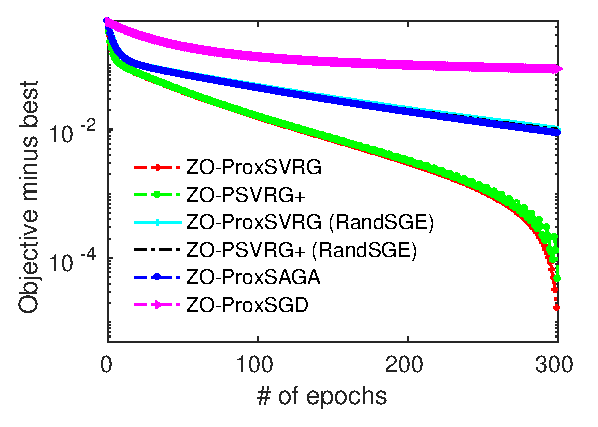
\includegraphics[width=0.23\linewidth]{Figures/binary/ijcnn1b50k1.eps}}%
\addtocounter{subfigure}{-4}
\subfloat{
\centering
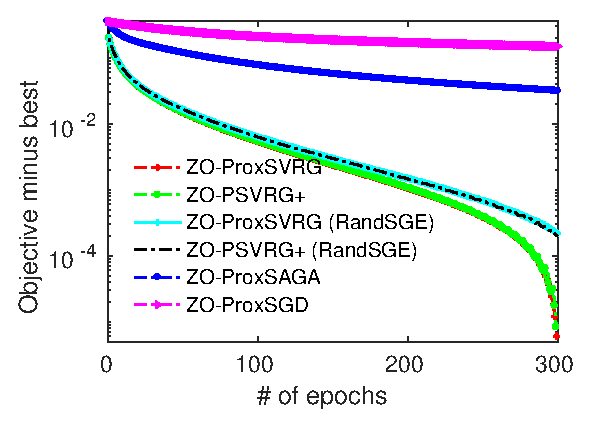
\includegraphics[width=0.23\linewidth]{Figures/binary/adultb50k1.eps}}%
\subfloat{
\centering
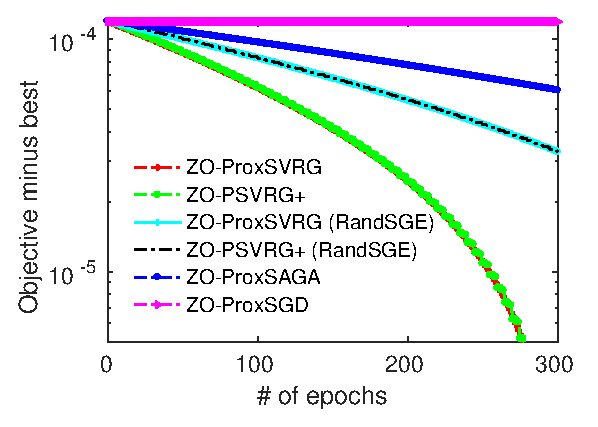
\includegraphics[width=0.23\linewidth]{Figures/binary/w8ab50k1.eps}}%
\subfloat{
\centering
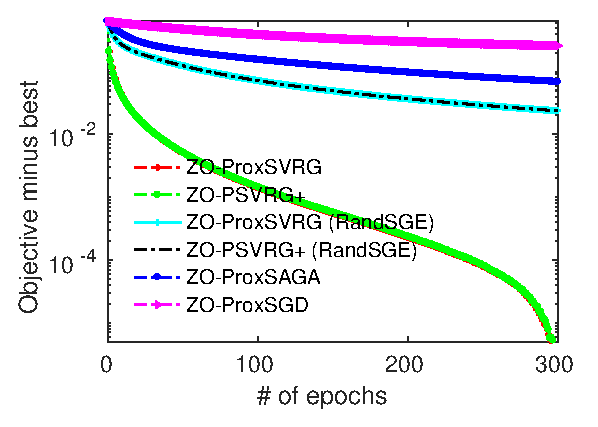
\includegraphics[width=0.23\linewidth]{Figures/binary/mnistb50k1.eps}}\\
\subfloat[ijcnn]{
\centering
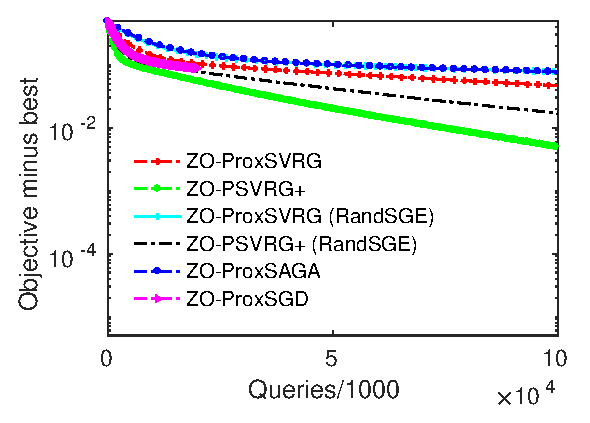
\includegraphics[width=0.23\linewidth]{Figures/binary/ijcnn1b50k2.eps}}%
\subfloat[comparison on covtype]{
\centering
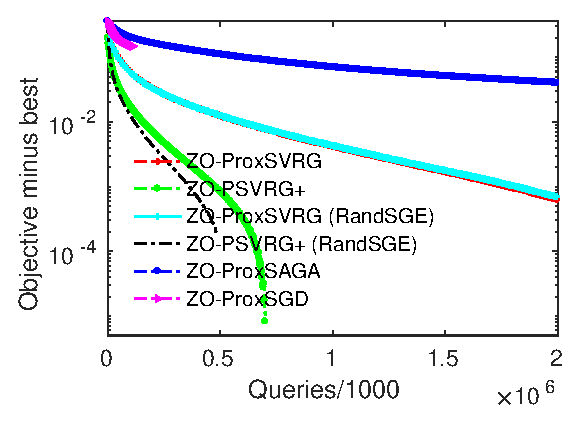
\includegraphics[width=0.23\linewidth]{Figures/binary/adultb50k2.eps}}%
\subfloat[w8a]{
\centering
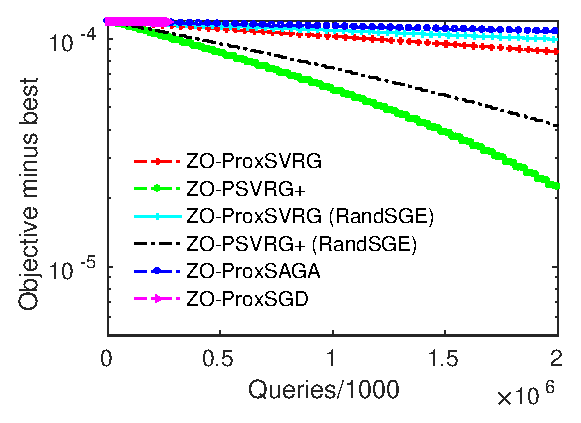
\includegraphics[width=0.23\linewidth]{Figures/binary/w8ab50k2.eps}}%
\subfloat[mnist]{
\centering
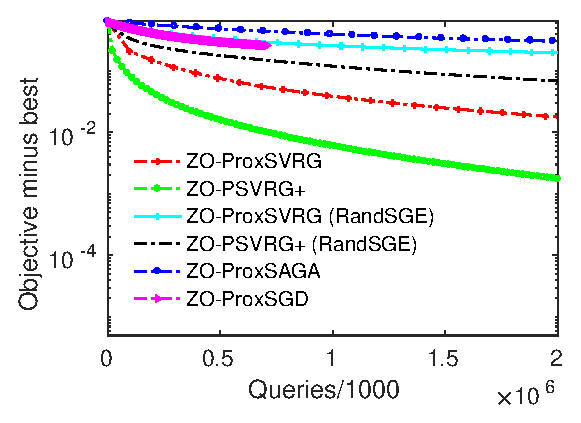
\includegraphics[width=0.23\linewidth]{Figures/binary/mnistb50k2.eps}}%
\setlength{\abovecaptionskip}{2pt}
\caption{Comparison of different zeroth-order algorithms for logistic regression loss residual $f(x) - f(x^*)$ versus the number of epochs (top) and ZO queries (bottom)}
\label{binary-fig}
\end{figure*}
In Figure \ref{binary-fig} (top), we show the training loss versus the number of epochs (i.e., iterations divided by the
epoch length $m = 30$). Note that ZO-PSVRG+ is evaluated using mix gradient CoordSGE \eqref{gradestcoord} and mix gradient RandSGE \eqref{gradestrand}.
Results in Figure \ref{binary-fig} (bottom) compare the performance of ZO-PSVRG+ with the variants of ZO variance reduced stochastic gradient descent described earlier in this section against the number of function queries. In these figures, we notice  a relatively faster convergence rate for ZO-PSVRG+ than the counterpart ZO-PSVRG+ (RandSGE). Note that ZO-ProxSVRG based on
our improved analysis have faster
convergence rate than ZO-ProxSAGA and also ZO-ProxSGD. On the other hand, the use of $\mathcal{B} = \lfloor{\frac{n}{5}}\rfloor$ in ZO-PSVRG+ significantly
improves ZO-ProxSVRG with respect to the number of ZO-queries (see Table \ref{table-compare}), leading to a non-dominant factor $O(I_{\{\mathcal{B} < n\}}/\mathcal{B})$ in the convergence rate of ZO-PSVRG+. Particularly ZO-PSVRG+ exhibits better performance in terms of number of function queries than ZO-ProxSAGA using CoordSGE.  The degradation in the convergence of ZO-ProxSAGA  is due to the requisite for small stepsizes $O(\frac{1}{d})$. Similarly, the large number of function queries to construct
coordinate-wise gradient estimates increases significantly the number of SZO queries for ZO-ProxSVRG. On the other hand, ZO-ProxSGD consumes an extremely large number of iterations while exhibiting marginal convergence compared with variance reduced algorithms. Thus, ZO-PSVRG+ obtains the best tradeoffs between the iteration and the function query complexity.





\subsection{Adversarial Attacks on Black-Box DNNs}
Adversarial 
examples in image classification are related to designing unperceptive perturbations such that they lead to misclassifying the target model by adding to the natural images. In the framework of zeroth-order attacks \cite{chen2017zoo,liu2018zeroth}, the model parameters are hidden and obtaining its gradient is not feasible, while only
the model evaluations are available. We can then consider the task of producing a universal adversarial
example with respect to $n$ natural images as an ZO optimization problem of the form \eqref{problem}.
More precisely, we apply the zeroth-order algorithms to obtain a global adversarial perturbation $x\in\R^d$ that could mislead the classifier on samples $\{a_i \in \R^d, y_i\in\mathbb{N} \}_{i=1}^n$. This problem can be specified as the following elastic-net attacks to black-box DNNs problem:
\begin{align}
\min_{x\in\R^d} \frac{1}{n} \sum_{i=1}^n& \max\{F_{y_i}(a_i^{adv}) - \max_{j\neq y_i}F_j(a_i^{adv}),0\}\notag\\
& + c\norm{a_i^{adv} - a_i}^2 + \lambda_1 \norm{x}_{1} + \lambda_2 \norm{x}^{2}\label{mnist-attack-loss}
\end{align}
where $a_i^{adv} = 0.5\tanh(\tanh^{-1}(2a_i)+x)$ and $\lambda_1$ and $\lambda_2$ are nonnegative parameters to obtain consistency between attack success rate, distortion and sparsity. Here $F(a) = \left[F_1(a),\ldots,F_K(a)\right]\in [0, 1]^K$ describes a trained DNN{\footnote{https://github.com/carlini/nn$\underline{~~}$robust$\underline{~~}$attacks}} for the MNIST handwritten digit classification, where $F_i(a)$ returns the prediction score of $i$-th class. The parameter $c$ in \eqref{mnist-attack-loss} compensates the rate of adversarial success and the distortion of adversarial examples. In our experiment, we set the regularization parameter  $c = 0.2$ and $\lambda_1 = \lambda_2  = 10^{-5}$.
\begin{figure}[htbp]
\subfloat[Loss vs iterations: $n = 10$]{
\centering
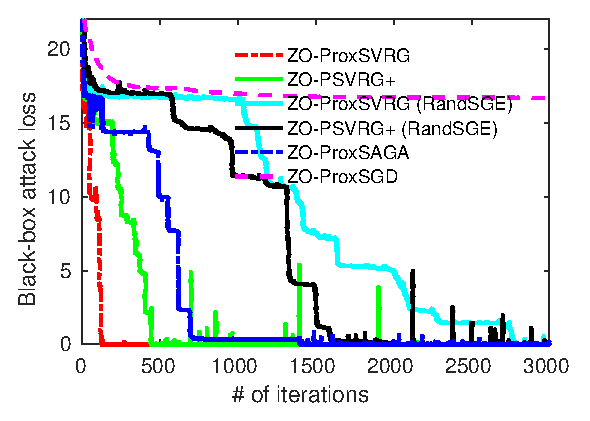
\includegraphics[width=0.44\linewidth]{Figures/attack/figiter.eps}}%
\subfloat[Loss vs queries: $n = 10$]{
\centering
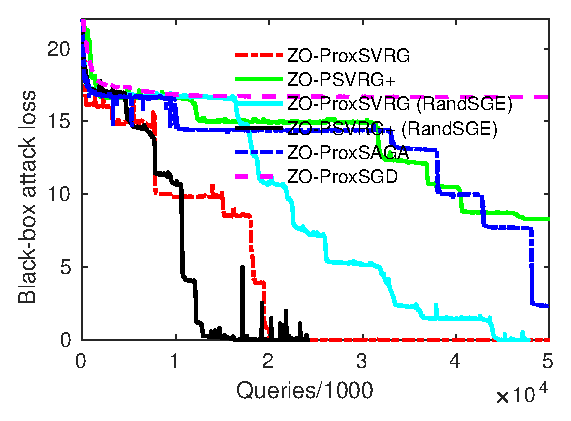
\includegraphics[width=0.44\linewidth]{Figures/attack/figquery.eps}}%
\setlength{\abovecaptionskip}{2pt}
\caption{Comparison of different zeroth-order algorithms for generating black-box adversarial examples from a black-box DNN}
\label{attack-fig}
\end{figure}
We perform two experiments by choosing $n = 10$ and $n=100$ images from the same class, and set the minibatch sizes, respectively $b=5$ and $b = 30$. We select the batch size $\mathcal{B} = \lfloor{\frac{n}{2}}\rfloor$ for ZO-PSVRG+.
Figure \ref{attack-fig} shows
the performance of different ZO algorithms considered in this paper. Our two algorithms ZO-PSVRG+ (RandSGE) and ZO-ProxSVRG (under our improved analysis) show better performance
both in convergence rate (iteration complexity) and function query complexity than ZO-ProxSGD
and ZO-ProxSAGA. The performance of ZO-PSVRG+ (CoordSGE) algorithm degrades due to large number of function queries for CoordSGE and the variance inherited by $\mathcal{B} \neq n$. 
ZO-PSVRG+ (RandSGE) shows faster convergence in the initial optimization stage, and more importantly, has much lower function query complexity, which is largely
due to efficient ZO queries for computing mix gradient \eqref{zo-grad-fo-rand} and  the $O(\frac{1}{\sqrt{d}})$-level stepsize required by ZO-PSVRG+ (RandSGE). ZO-ProxSAGA and ZO-PSVRG+ (CoordSGE) exhibit relatively similar convergence behaviors. Furthermore, the convergence performance of ZO-ProxSGD is poor compared to other algorithms due to not using variance reduced techniques. 
\iffalse
\ref{fig:FSVRG_compare} shows the convergence of the objective function with respect to CPU time and the number of iterations. 
\begin{figure}[htbp]
\subfloat[a]{
\centering
\includegraphics[width=0.44\linewidth]{Figures/figure_logistic_rcv_update_32_time.eps}}%
\hfill
\subfloat[b]{
\centering
\includegraphics[width=0.44\linewidth]{Figures/figure_logistic_rcv_update_32_iteration.eps}}%
\caption{Figure(a) is convergence of objective value vs. time; Figure(b) is comparison of the objective function vs. iteration for different algorithms.}
\label{fig:FSVRG_compare}
\end{figure}
\fi


\section{Conclusion}
In this paper, we developed a novel analysis for two zeroth-order variance-reduced proximal algorithms named 
ZO-PSVRG+ and ZO-PSVRG+ (RangSGE). We prove that ZO-PSVRG+ improves and generalizes the analysis for several well-known convergence
results, e.g., ZO-ProxSVRG. Compared with ZO-SVRG-Coord-Rand  \cite{ji2019improved}, our analysis allows single minibatch size and larger
stepsizes while improving the function query complexity. Moreover, for nonconvex functions under Polyak-Łojasiewicz condition, we prove that ZO-PSVRG+
obtains global linear convergence for a wide range of minibatch sizes without restart. Experimental results demonstrate the effectiveness of our novel approaches compared to other state-of-the-art algorithms.

%\section{Introduction}
%% The very first letter is a 2 line initial drop letter followed
%% by the rest of the first word in caps.
%% 
%% form to use if the first word consists of a single letter:
%% \IEEEPARstart{A}{demo} file is ....
%% 
%% form to use if you need the single drop letter followed by
%% normal text (unknown if ever used by the IEEE):
%% \IEEEPARstart{A}{}demo file is ....
%% 
%% Some journals put the first two words in caps:
%% \IEEEPARstart{T}{his demo} file is ....
%% 
%% Here we have the typical use of a "T" for an initial drop letter
%% and "HIS" in caps to complete the first word.
%\IEEEPARstart{T}{his} demo file is intended to serve as a ``starter file''
%for IEEE journal papers produced under \LaTeX\ using
%IEEEtran.cls version 1.8b and later.
%% You must have at least 2 lines in the paragraph with the drop letter
%% (should never be an issue)
%I wish you the best of success.
%
%\hfill mds
% 
%\hfill August 26, 2015
%
%\subsection{Subsection Heading Here}
%Subsection text here.
%
%% needed in second column of first page if using \IEEEpubid
%%\IEEEpubidadjcol
%
%\subsubsection{Subsubsection Heading Here}
%Subsubsection text here.


% An example of a floating figure using the graphicx package.
% Note that \label must occur AFTER (or within) \caption.
% For figures, \caption should occur after the \includegraphics.
% Note that IEEEtran v1.7 and later has special internal code that
% is designed to preserve the operation of \label within \caption
% even when the captionsoff option is in effect. However, because
% of issues like this, it may be the safest practice to put all your
% \label just after \caption rather than within \caption{}.
%
% Reminder: the "draftcls" or "draftclsnofoot", not "draft", class
% option should be used if it is desired that the figures are to be
% displayed while in draft mode.
%
%\begin{figure}[!t]
%\centering
%\includegraphics[width=2.5in]{myfigure}
% where an .eps filename suffix will be assumed under latex, 
% and a .pdf suffix will be assumed for pdflatex; or what has been declared
% via \DeclareGraphicsExtensions.
%\caption{Simulation results for the network.}
%\label{fig_sim}
%\end{figure}

% Note that the IEEE typically puts floats only at the top, even when this
% results in a large percentage of a column being occupied by floats.


% An example of a double column floating figure using two subfigures.
% (The subfig.sty package must be loaded for this to work.)
% The subfigure \label commands are set within each subfloat command,
% and the \label for the overall figure must come after \caption.
% \hfil is used as a separator to get equal spacing.
% Watch out that the combined width of all the subfigures on a 
% line do not exceed the text width or a line break will occur.
%
%\begin{figure*}[!t]
%\centering
%\subfloat[Case I]{\includegraphics[width=2.5in]{box}%
%\label{fig_first_case}}
%\hfil
%\subfloat[Case II]{\includegraphics[width=2.5in]{box}%
%\label{fig_second_case}}
%\caption{Simulation results for the network.}
%\label{fig_sim}
%\end{figure*}
%
% Note that often IEEE papers with subfigures do not employ subfigure
% captions (using the optional argument to \subfloat[]), but instead will
% reference/describe all of them (a), (b), etc., within the main caption.
% Be aware that for subfig.sty to generate the (a), (b), etc., subfigure
% labels, the optional argument to \subfloat must be present. If a
% subcaption is not desired, just leave its contents blank,
% e.g., \subfloat[].


% An example of a floating table. Note that, for IEEE style tables, the
% \caption command should come BEFORE the table and, given that table
% captions serve much like titles, are usually capitalized except for words
% such as a, an, and, as, at, but, by, for, in, nor, of, on, or, the, to
% and up, which are usually not capitalized unless they are the first or
% last word of the caption. Table text will default to \footnotesize as
% the IEEE normally uses this smaller font for tables.
% The \label must come after \caption as always.
%
%\begin{table}[!t]
%% increase table row spacing, adjust to taste
%\renewcommand{\arraystretch}{1.3}
% if using array.sty, it might be a good idea to tweak the value of
% \extrarowheight as needed to properly center the text within the cells
%\caption{An Example of a Table}
%\label{table_example}
%\centering
%% Some packages, such as MDW tools, offer better commands for making tables
%% than the plain LaTeX2e tabular which is used here.
%\begin{tabular}{|c||c|}
%\hline
%One & Two\\
%\hline
%Three & Four\\
%\hline
%\end{tabular}
%\end{table}


% Note that the IEEE does not put floats in the very first column
% - or typically anywhere on the first page for that matter. Also,
% in-text middle ("here") positioning is typically not used, but it
% is allowed and encouraged for Computer Society conferences (but
% not Computer Society journals). Most IEEE journals/conferences use
% top floats exclusively. 
% Note that, LaTeX2e, unlike IEEE journals/conferences, places
% footnotes above bottom floats. This can be corrected via the
% \fnbelowfloat command of the stfloats package.



%
%\section{Conclusion}
%The conclusion goes here.





% if have a single appendix:
%\appendix[Proof of the Zonklar Equations]
% or
%\appendix  % for no appendix heading
% do not use \section anymore after \appendix, only \section*
% is possibly needed

% use appendices with more than one appendix
% then use \section to start each appendix
% you must declare a \section before using any
% \subsection or using \label (\appendices by itself
% starts a section numbered zero.)
%


%\appendices
%\section{Proof of the First Zonklar Equation}
%Appendix one text goes here.
%
%% you can choose not to have a title for an appendix
%% if you want by leaving the argument blank
%\section{}
%Appendix two text goes here.
%
%
%% use section* for acknowledgment
%\section*{Acknowledgment}
%
%
%The authors would like to thank...


% Can use something like this to put references on a page
% by themselves when using endfloat and the captionsoff option.
\ifCLASSOPTIONcaptionsoff
  \newpage
\fi



% trigger a \newpage just before the given reference
% number - used to balance the columns on the last page
% adjust value as needed - may need to be readjusted if
% the document is modified later
%\IEEEtriggeratref{8}
% The "triggered" command can be changed if desired:
%\IEEEtriggercmd{\enlargethispage{-5in}}

% references section

% can use a bibliography generated by BibTeX as a .bbl file
% BibTeX documentation can be easily obtained at:
% http://mirror.ctan.org/biblio/bibtex/contrib/doc/
% The IEEEtran BibTeX style support page is at:
% http://www.michaelshell.org/tex/ieeetran/bibtex/
\bibliographystyle{IEEEtran}
% argument is your BibTeX string definitions and bibliography database(s)
\bibliography{GTA}
%
% <OR> manually copy in the resultant .bbl file
% set second argument of \begin to the number of references
% (used to reserve space for the reference number labels box)
%\begin{thebibliography}{1}
%
%\bibitem{IEEEhowto:kopka}
%H.~Kopka and P.~W. Daly, \emph{A Guide to \LaTeX}, 3rd~ed.\hskip 1em plus
%  0.5em minus 0.4em\relax Harlow, England: Addison-Wesley, 1999.
%
%\end{thebibliography}

% biography section
% 
% If you have an EPS/PDF photo (graphicx package needed) extra braces are
% needed around the contents of the optional argument to biography to prevent
% the LaTeX parser from getting confused when it sees the complicated
% \includegraphics command within an optional argument. (You could create
% your own custom macro containing the \includegraphics command to make things
% simpler here.)
%\begin{IEEEbiography}[{\includegraphics[width=1in,height=1.25in,clip,keepaspectratio]{mshell}}]{Michael Shell}
% or if you just want to reserve a space for a photo:

%\begin{IEEEbiography}{Michael Shell}
%Biography text here.
%\end{IEEEbiography}
%
%% if you will not have a photo at all:
%\begin{IEEEbiographynophoto}{John Doe}
%Biography text here.
%\end{IEEEbiographynophoto}
%
%% insert where needed to balance the two columns on the last page with
%% biographies
%%\newpage
%
%\begin{IEEEbiographynophoto}{Jane Doe}
%Biography text here.
%\end{IEEEbiographynophoto}

% You can push biographies down or up by placing
% a \vfill before or after them. The appropriate
% use of \vfill depends on what kind of text is
% on the last page and whether or not the columns
% are being equalized.

%\vfill

% Can be used to pull up biographies so that the bottom of the last one
% is flush with the other column.
%\enlargethispage{-5in}



% that's all folks
\end{document}


